% Options for packages loaded elsewhere
\PassOptionsToPackage{unicode}{hyperref}
\PassOptionsToPackage{hyphens}{url}
%
\documentclass[
]{book}
\title{Guide for Trainers - COVID-19 Lebanon}
\author{Robert ten Hove}
\date{2021-06-24}

\usepackage{amsmath,amssymb}
\usepackage{lmodern}
\usepackage{iftex}
\ifPDFTeX
  \usepackage[T1]{fontenc}
  \usepackage[utf8]{inputenc}
  \usepackage{textcomp} % provide euro and other symbols
\else % if luatex or xetex
  \usepackage{unicode-math}
  \defaultfontfeatures{Scale=MatchLowercase}
  \defaultfontfeatures[\rmfamily]{Ligatures=TeX,Scale=1}
\fi
% Use upquote if available, for straight quotes in verbatim environments
\IfFileExists{upquote.sty}{\usepackage{upquote}}{}
\IfFileExists{microtype.sty}{% use microtype if available
  \usepackage[]{microtype}
  \UseMicrotypeSet[protrusion]{basicmath} % disable protrusion for tt fonts
}{}
\makeatletter
\@ifundefined{KOMAClassName}{% if non-KOMA class
  \IfFileExists{parskip.sty}{%
    \usepackage{parskip}
  }{% else
    \setlength{\parindent}{0pt}
    \setlength{\parskip}{6pt plus 2pt minus 1pt}}
}{% if KOMA class
  \KOMAoptions{parskip=half}}
\makeatother
\usepackage{xcolor}
\IfFileExists{xurl.sty}{\usepackage{xurl}}{} % add URL line breaks if available
\IfFileExists{bookmark.sty}{\usepackage{bookmark}}{\usepackage{hyperref}}
\hypersetup{
  pdftitle={Guide for Trainers - COVID-19 Lebanon},
  pdfauthor={Robert ten Hove},
  hidelinks,
  pdfcreator={LaTeX via pandoc}}
\urlstyle{same} % disable monospaced font for URLs
\usepackage{longtable,booktabs,array}
\usepackage{calc} % for calculating minipage widths
% Correct order of tables after \paragraph or \subparagraph
\usepackage{etoolbox}
\makeatletter
\patchcmd\longtable{\par}{\if@noskipsec\mbox{}\fi\par}{}{}
\makeatother
% Allow footnotes in longtable head/foot
\IfFileExists{footnotehyper.sty}{\usepackage{footnotehyper}}{\usepackage{footnote}}
\makesavenoteenv{longtable}
\usepackage{graphicx}
\makeatletter
\def\maxwidth{\ifdim\Gin@nat@width>\linewidth\linewidth\else\Gin@nat@width\fi}
\def\maxheight{\ifdim\Gin@nat@height>\textheight\textheight\else\Gin@nat@height\fi}
\makeatother
% Scale images if necessary, so that they will not overflow the page
% margins by default, and it is still possible to overwrite the defaults
% using explicit options in \includegraphics[width, height, ...]{}
\setkeys{Gin}{width=\maxwidth,height=\maxheight,keepaspectratio}
% Set default figure placement to htbp
\makeatletter
\def\fps@figure{htbp}
\makeatother
\setlength{\emergencystretch}{3em} % prevent overfull lines
\providecommand{\tightlist}{%
  \setlength{\itemsep}{0pt}\setlength{\parskip}{0pt}}
\setcounter{secnumdepth}{5}
\usepackage{booktabs}
\ifLuaTeX
  \usepackage{selnolig}  % disable illegal ligatures
\fi
\ifXeTeX
  % Load bidi as late as possible as it modifies e.g. graphicx
  \usepackage{bidi}
\fi
\ifPDFTeX
  \TeXXeTstate=1
  \newcommand{\RL}[1]{\beginR #1\endR}
  \newcommand{\LR}[1]{\beginL #1\endL}
  \newenvironment{RTL}{\beginR}{\endR}
  \newenvironment{LTR}{\beginL}{\endL}
\fi

\begin{document}
\maketitle

{
\setcounter{tocdepth}{1}
\tableofcontents
}
\hypertarget{foreword}{%
\chapter{Foreword}\label{foreword}}

This guide for teachers is part of the EU project 73 action plan for the
COVID19 emergency response activities in Lebanon. A major part of action
plan has to be delivered by trainees of first responders. The guide
forms a handbook for the trainers to deliver the training on COVID19
emergency response, in particular for setting-up and operating Rapid Testing Facilities.


\includegraphics{images/CoE.jpeg}\\
\textbf{Trainers specification:}

To train the content of the COVID19 modules, trainers should be
selected. Good teaching skills is key in transferring knowledge. As the
content is taught to first responders, it is key to have a confident and
hands-on teacher delivering the training.

\textbf{Minimum qualifications:}

\begin{itemize}
\item
  Good training skills are key in transferring knowledge.
\item
  Professionally connected to community health service provider
\item
  Computer literate
\end{itemize}

\textbf{Additional relevant experiences:}

\begin{itemize}
\item
  Background in C, B and/or RN
\item
  Experience in clinical diagnostic settings.
\end{itemize}

\textbf{Acknowledgements\\
}Material for the modules was contributed by the Amsterdam Municipality
Health Services (GGD-Amsterdam), the COVID19 testing center in
Kranenburg, Germany and various staff-members at the RIVM.

\hypertarget{executive-summary}{%
\section{Executive Summary}\label{executive-summary}}

This guide for trainers contains an introduction of the curriculum,
guidance on the curriculum structure and objectives and an overview of
the modules and individual topics therein. The COVID19 curriculum covers
the following modules:

Module I: Introduction

Module II: Types of Rapid Tests

Module III: Validation of Test Kits

Module IV: Quality Management in Testing Center

Module V: Set-up and Workflow in Testing Center

Module VI: Practical training

\hypertarget{intro}{%
\chapter{Introduction}\label{intro}}

\hypertarget{background}{%
\section{Background}\label{background}}

In Lebanon, the Coronavirus disease (COVID-19) pandemic has disrupted
the lives of inhabitants and forced the country to devise public health
policies to reduce the pace of transmission. The socio-political
tensions and the large refugee populations have increased the disease
burden of COVID-19. The support of first responders are particularly
necessary to implement effective disease control measures to reduce
SARS-CoV-2 persistence and transmission. Measures that are designed to
reduce aerosol transmission within the population must be implemented,
which include universal masking and regular, widespread testing to
identify and isolate infected symptomatic and asymptomatic individuals.

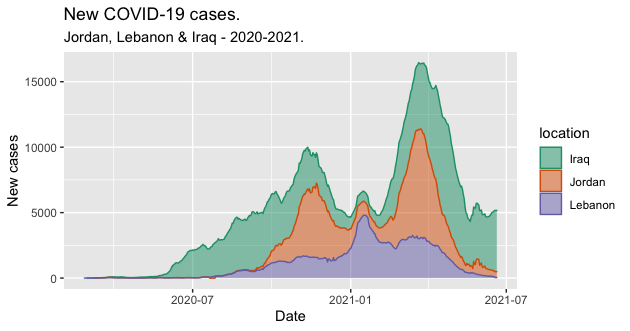
\includegraphics{images/covid19_ME.png}

\emph{Source: \href{https://ourworldindata.org/coronavirus}{Our world in data}}

Testing of SARS-CoV-2 is central to COVID-19 management and relies
heavily on rt-PCR technology. For public health measures, another
approach is needed in which the focus is to determine within minutes
whether a person is infectious, instead of determining if a person is
carrier of the virus (nucleic acid).

For rapid and cheap SARS-CoV-2 testing, a large number of rapid tests
are offered on the global market. The reliability of the test should
undergo thorough examination before they are allowed for use. After
validation, test kits should be monitored continuously.

The training explains the different types of rapid tests. The
participants will learn to setup and perform a validation of a rapid
test. Secondly, the participants will learn to conduct continues quality
monitoring. Finally, the participants will learn to setup save and
efficient workflows in testing-centres.

This guide for trainers describes the material and activities that can
be applied to achieve the optimal outcomes when transferring knowledge
and practices on controlling COVID-19.

\hypertarget{overview}{%
\chapter{Overview}\label{overview}}

Summary overview of his guide.

Overview of content

\begin{longtable}[]{@{}
  >{\raggedright\arraybackslash}p{(\columnwidth - 4\tabcolsep) * \real{0.25}}
  >{\raggedright\arraybackslash}p{(\columnwidth - 4\tabcolsep) * \real{0.51}}
  >{\raggedright\arraybackslash}p{(\columnwidth - 4\tabcolsep) * \real{0.24}}@{}}
\toprule
\endhead
\textbf{Length} & \begin{minipage}[t]{\linewidth}\raggedright
\textbf{Content}
\end{minipage} & \begin{minipage}[t]{\linewidth}\raggedright
\textbf{Duration}
\end{minipage} \\
\textbf{Practical information} & Facilities, equipment, target audience & \emph{NA} \\
\textbf{Presentations} & \begin{minipage}[t]{\linewidth}\raggedright
\begin{itemize}
\item
  Module II - Types of SARS-CoV-2 Tests
\item
  Quiz questions
\item
  FAQ
\end{itemize}
\end{minipage} & 13 minutes presentation \\
& \begin{minipage}[t]{\linewidth}\raggedright
\begin{itemize}
\item
  Module II - Types of SARS-CoV-2 Tests
\item
  Quiz questions
\item
  FAQ
\end{itemize}
\end{minipage} & 14 minutes presentation \\
& \begin{minipage}[t]{\linewidth}\raggedright
\begin{itemize}
\item
  Module III - Validation of test kits
\item
  Quiz questions
\item
  FAQ
\end{itemize}
\end{minipage} & 12 minutes presentation \\
& \begin{minipage}[t]{\linewidth}\raggedright
\begin{itemize}
\item
  Module IV - Quality Management
\item
  Quiz questions
\item
  FAQ
\end{itemize}
\end{minipage} & 15 minutes presentation \\
& \begin{minipage}[t]{\linewidth}\raggedright
\begin{itemize}
\item
  Module V - Workflow
\item
  Quiz questions
\item
  FAQ
\end{itemize}
\end{minipage} & 14 minutes presentation \\
\textbf{Practical trainings} & Introduction to Practical training & 10-20 minutes \\
& Donning \& Doffing & 1 hour \\
& Sample taking \& rapid test & 1 hour and 30 minutes \\
& Standard Operation Procedures & 1 hour \\
& Root Cause Analysis & 1 hour \\
& Design test site & 1 hour \\
& Setup test site & 45 minutes \\
& Simulate test site & 1 hour and 30 minutes \\
\textbf{Appendix} & Materials, supplies, and kits for practical trainings & \emph{NA} \\
\bottomrule
\end{longtable}

\hypertarget{trainer_info}{%
\chapter{Practical information}\label{trainer_info}}

\textbf{Presentations} can be provided for participants in person and/or
online. For \textbf{workshops}, it is recommended for optimal learning
experience and management that the number of participants do not exceed
five (maybe six) participants per instructor. This number is small
enough for all participants to be fully engaged, yet large enough for a
variety of experiences and viewpoints to be represented.

\hypertarget{facs}{%
\section{Facilities and equipment}\label{facs}}

For in-person trainings, the environment should be large enough for
training, discussion and the simulation. The trainings or workshops can
be held in a well-lit, ventilated, distraction-free classroom with
sufficient tables and chairs, and conveniently located outlets for a
computer and projection monitor. To facilitate discussion and
interaction among participants, tables should be arranged in a
semi-circle, or classroom-style, giving all participants an unobstructed
view of the projection monitor. Avoid overcrowding. It is important to
consider social distancing requirements when preparing the training
venue and limit the training to smaller groups. Bottled water and
glasses should be made available on each table. Facilities must be
available for participants to clean their hands (with soap and water or
an alcohol-based hand rub). Refer to local guidelines for measures that
must be in place for workshops of this nature.

Make arrangements well in advance of the workshop to procure or secure
the necessary materials, supplies and kits. Do not forget to arrange for
transport of these items to the workshop site.

\hypertarget{target}{%
\section{Target audience}\label{target}}

The training can be provided to lab technicians, lab managers, first
responders, quality managers, or anyone involved in SARS-CoV-2
screening. The setup and content of the training is adequate for all
backgrounds and levels of expertise. The training participants should
have general knowledge of diagnostic settings and familiar with general
aspects of infectious diseases and hygiene.

\hypertarget{course-language}{%
\section{Course Language}\label{course-language}}

Training material are provided in English. The documents and forms can
be edited for translation into different languages.

\hypertarget{presentations}{%
\chapter{Presentations}\label{presentations}}

\hypertarget{introduction}{%
\section{Introduction}\label{introduction}}

The presentations and training material are deployed online on the RIVM
\textbf{\href{https://rivm-academie.cappagile.com/s/DcYnbt1tmyFU9GKQWUEHgg}{Capp-Agile website}}
Participants can access the modules after registration.

A face-to-face meetup can be organised for the participants for in-depth
and interactive training, and for discussions with the local training.
The trainer can use the presentation sheets and the narrative to compose
their own presentation(s). Presentation can be alternated with practical
exercises listed in section `\textbf{Practical training}.'

The following section lists the content of the presentations, the
narratives, quiz questions and frequently asked questions.

\hypertarget{M2}{%
\section{Module II - Types of SARS-CoV-2 Tests}\label{M2}}

\hypertarget{content}{%
\subsection{Content}\label{content}}

\begin{longtable}[]{@{}
  >{\raggedright\arraybackslash}p{(\columnwidth - 2\tabcolsep) * \real{0.25}}
  >{\raggedright\arraybackslash}p{(\columnwidth - 2\tabcolsep) * \real{0.74}}@{}}
\toprule
\endhead
\textbf{Length} & 13 minutes presentation \\
\textbf{Learning
goals} & The participants can:

\textbf{Describe} different types of rapid tests for
SARS-CoV-2 detection.

\textbf{Argue} the (dis/)advantages of the types of
tests

\textbf{Illustrate} criteria that can be applied to
rapids tests

\textbf{Argue} why a validation procedure is needed. \\
\textbf{Summary} & The presentation starts with illustrating the
importance of validating new medical devices
before they are applied. Does the rapid test
fulfill its' role in
its' purpose?

List types of diagnostics and its characteristics:
1) PCR, 2) Antigen testing, 3) Serology, 4)
Biomarkers. Characteristics include price,
equipment, sensitivity/specificity, type of
sample.

As an example, criteria are listed to which both
the manufacturer and the tests characteristics
need to comply with. \\
\textbf{Tools \&
setup} & Ask participants to turn of (sound of) mobile
telephones

Explain if and when questions can be asked.

Relevant literature. PowerPoint slides. Presenter
in front of slides. Small quiz for recap. \\
\bottomrule
\end{longtable}

\hypertarget{narrative}{%
\subsection{Narrative}\label{narrative}}

\textbf{Sheet 02 - Introduction}

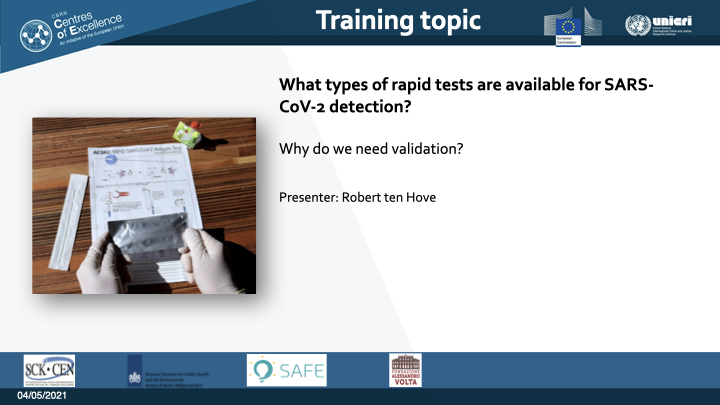
\includegraphics{images/m02/m02_types_of_rapid_tests_final.002.jpeg}

In this module, I will discuss different types of rapid tests for the
detection of Corona infections. Countries across the world are facing
difficulties containing COVID outbreaks. Testing and contact tracing
have a large impact on reducing transmission of the virus. To strengthen
the identification of people carrying the virus, there is a large demand
for rapid tests, which are also called lateral flow tests. Manufacturers
are competing on the market with different types of rapid tests,
assuring that their product is of the highest quality. So, if
manufactures are confident in the performance of their tests, do we need
to validated them ourselves? Before we handle this question, let us
first examine what types of rapid tests are available and what their
advantages and disadvantages are, and what they can be used for.

\begin{center}\rule{0.5\linewidth}{0.5pt}\end{center}

\textbf{Sheet 03 -- Learning Objectives}

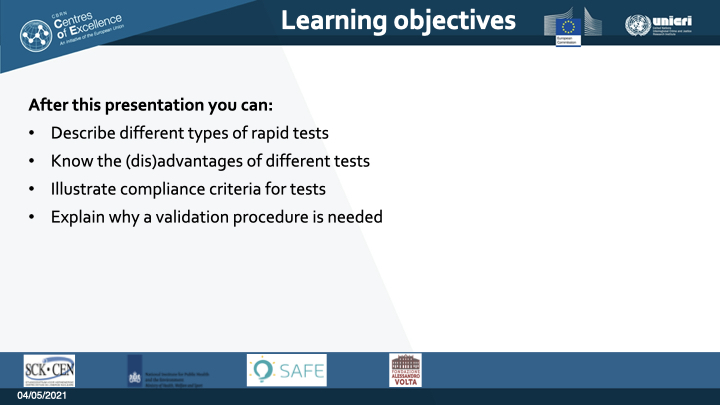
\includegraphics{images/m02/m02_types_of_rapid_tests_final.003.jpeg}

This presentation will take around 15 minutes. We will discuss the basic
principles of current Coronavirus tests and their advantages and
disadvantages. Different types of tests also have different compliance
criteria. The type of compliance criteria depends on how and for what
the test is used for. By the end of this module, you will understand why
test validation is needed. In the next module, we will learn about the
validation procedure itself.

\begin{center}\rule{0.5\linewidth}{0.5pt}\end{center}

\textbf{Sheet 04 -- Why validating?}

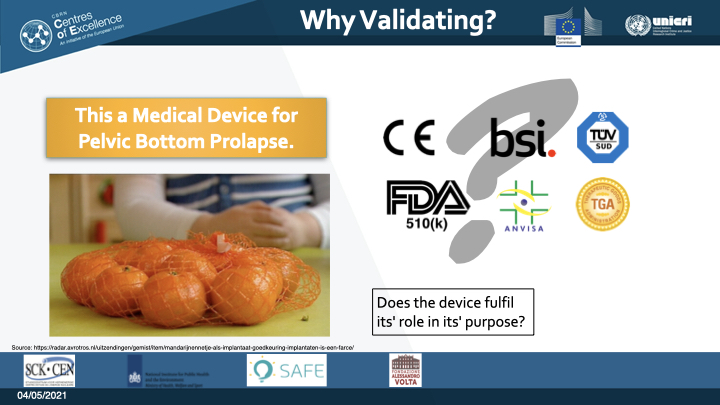
\includegraphics{images/m02/m02_types_of_rapid_tests_final.004.jpeg}

Scandals on inferior medical devices are unfortunately common. How is it
possible that such devices are still being sold? How does this system
work and where do the responsibilities of different stakeholders start
and end?

As an example, in 2014, journalists made up a medical device, a Pelvic
Floor Net for the treatment of Pelvic Organ Prolapse. The product was a
fruit net for oranges. The journalists wrote a brochure and a technical
briefing for it. The conclusion was that their product met the
certificate requirements for medical devices and was allowed to to be
sold on the market. This is an extreme example, but it does expose the
shortcomings of regulatory affairs. That being said, if regulatory
affairs are too strict, it would be very hard to manage outbreaks such
as the one we are facing now.

For diagnostic tests being bought to market during the ongoing COVID-19
outbreak, quality control markings do not always guarantee a reliable
test as one type of test may work better in one setting and not in
another. Therefore, the test needs to be checked, or validated, to see
if it works in a slightly different setting and circumstance.

\begin{center}\rule{0.5\linewidth}{0.5pt}\end{center}

\textbf{Sheet 05 -- Types of Tests I}

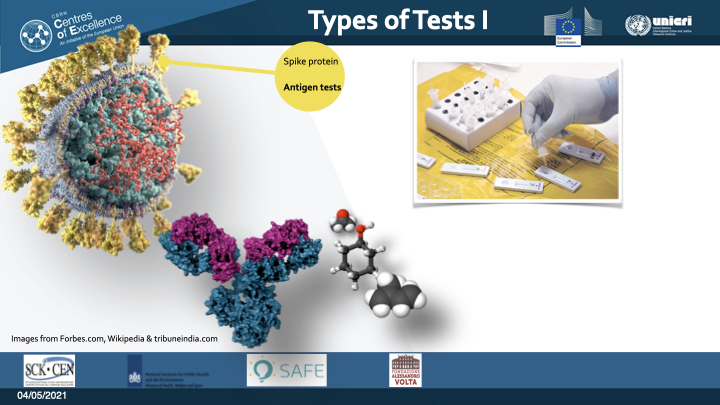
\includegraphics{images/m02/m02_types_of_rapid_tests_final.005.jpeg}

Different types of SARS-CoV-2 tests have different purposes.

In general, there are four types of tests for the detection of
SARS-CoV-2. On the left, you see a cross-section of the Coronavirus. The
virus particle has these yellow spikes on the outer membrane sticking
out. These spikes can be captured by antibodies that are attached to a
surface and subsequently coloured with a dye. A well-known example are
these rapid lateral flow tests. (\emph{Show rapid test for the camera}).

\begin{center}\rule{0.5\linewidth}{0.5pt}\end{center}

\textbf{Sheet 06 -- Types of Tests II}

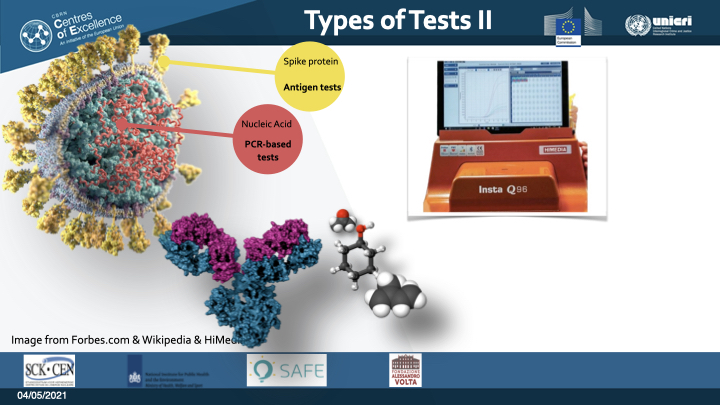
\includegraphics{images/m02/m02_types_of_rapid_tests_final.006.jpeg}

These spikes are on the outside. To reach the inside of the virus, the
particle needs to be treated with specific reagents in a test tube. The
released genetic material of the virus can then be detected using the
Polymerase Chain Reaction analysis, or PCR test.

\begin{center}\rule{0.5\linewidth}{0.5pt}\end{center}

\textbf{Sheet 07 -- Types of Tests III}

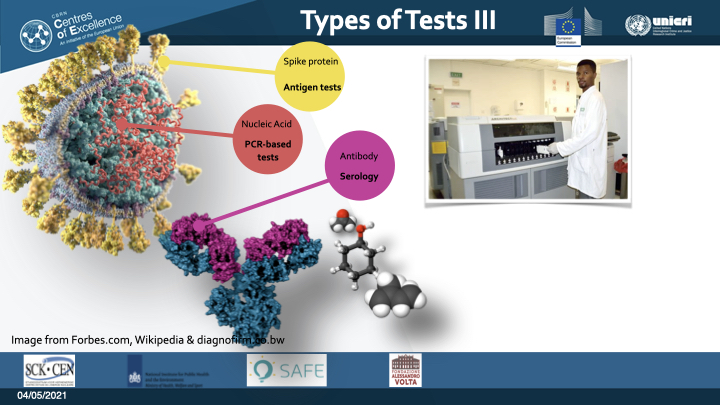
\includegraphics{images/m02/m02_types_of_rapid_tests_final.007.jpeg}

In a later stage of virus infection, the human body\RL{'}s
immune system is catching up with the infection and is releasing
specific antibodies in the bloodstream. These specific antibodies can be
detected with the so called serology tests. This is an indirect
detection approach for exposure to the virus as it detects human
produced antibodies and does not detect the virus itself.

\begin{center}\rule{0.5\linewidth}{0.5pt}\end{center}

\textbf{Sheet 08 -- Types of Tests IV}

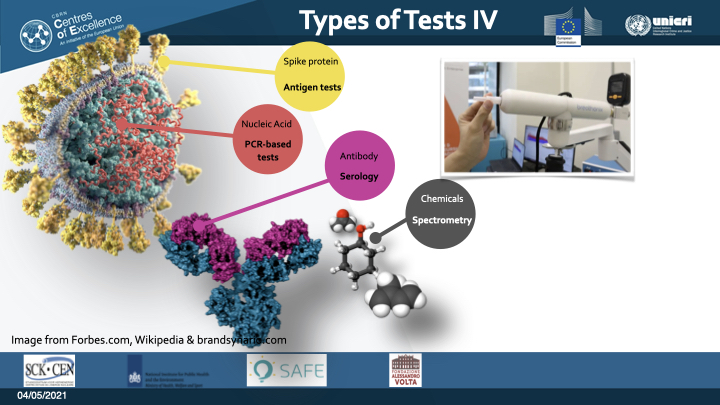
\includegraphics{images/m02/m02_types_of_rapid_tests_final.008.jpeg}

Other kinds of molecules or biomarkers are released by the human body
during an infection. These molecules can be detected and recognized with
sensitive equipment. For example, spectrometry analyzers are used for
the detection of specific quantities of small volatile molecules such as
acetone, ethanol, and others. Other biomarker tests are biochemical
tests include C‐reactive protein, measures of anticoagulation or blood
clotting, and immune cells such as white blood cell count. Then there
also imaging-biomarkers, such as X-ray or CT-scan. These are commonly
available tests and may be helpful for the triage of people with
possible COVID‐19 in imaging the lungs

Antigen and PCR tests can directly detect SARS-CoV-2 viral particles,
while serology and biomarkers are indirect detection methods and rely on
how the human body reacts to infection. They each have their advantages
and disadvantages, depending on what they are exactly used for.

\begin{center}\rule{0.5\linewidth}{0.5pt}\end{center}

\textbf{Sheet 09 -- Characteristics I}

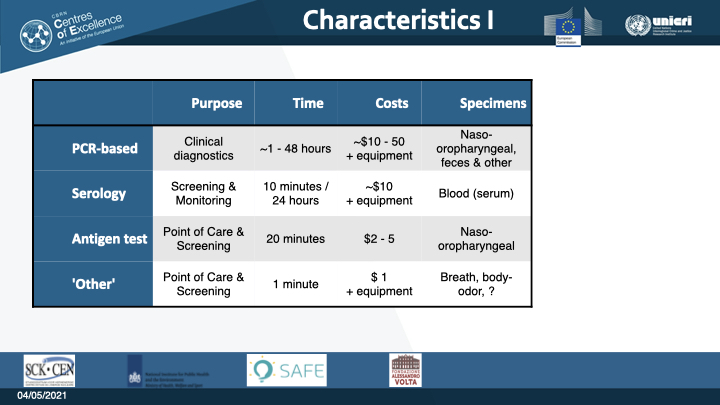
\includegraphics{images/m02/m02_types_of_rapid_tests_final.009.jpeg}

Let's compare these different types of tests.

Molecular or PCR-based tests are considered the gold standard. They are
versatile and the most reliable test for diagnosing covid patients.
Usually, these tests take a day: samples need to be transported to a
laboratory. Then the samples are processed, analyzed, checked, and
double-checked. Test reagents and equipment are expensive. Therefore, a
PCR test is only cost-effective when they are performed in large
quantities. Some PCR tests are less expensive or quicker, such as LAMP
and the GeneXpert. Still, these tests require specialized expertise and
lab equipment.

Serology is less expensive compared to molecular tests. In general,
serology is not used for the first diagnosis of Covid infection.
Antibody tests are likely to be available in laboratory form using
enzyme‐linked immunosorbent assay, or ELISA methods. But also as a
point‐of‐care test, using one or two spots of blood from a thumb prick
on a testing strip. It takes around 10 minutes for a positive answer.

Contrary to the antigen test. They are quick, cheap, and require little
training. The price, however, is that these rapid antigen tests are less
reliable.

Several other rapid tests are being developed, validated, and applied.
It ranges from breath analyzers to sniffing insect bees. I have grouped
these with `\emph{Others}.'

Choosing the right testing method depends on the objective of the test
and the available resources. Is for diagnosing a patient? Or for
monitoring donated blood units?

\begin{center}\rule{0.5\linewidth}{0.5pt}\end{center}

\textbf{Sheet 10 -- Characteristics II}

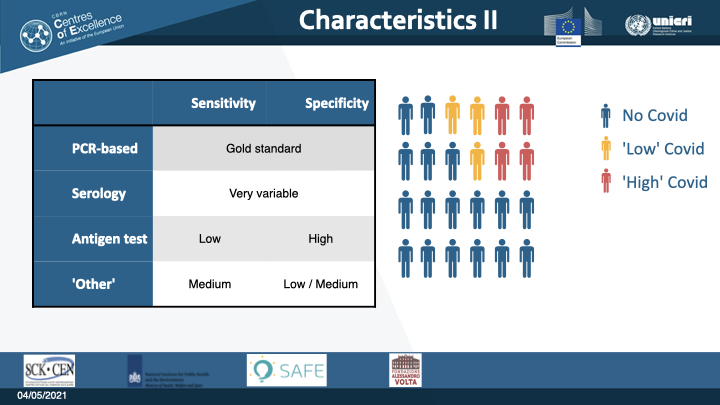
\includegraphics{images/m02/m02_types_of_rapid_tests_final.010.jpeg}

The most important indicators for the reliability of a test, are the
sensitivity, and specificity of the test. Let\RL{'}s imagine we
have a population. Most of them, the blue ones, do not carry the
Coronavirus. The yellow ones carry the virus but don\RL{'}t know
this yet. The number of viruses they have is very low and they do not
feel sick.

The red ones have high viral loads and are really sick with symptoms.

\begin{center}\rule{0.5\linewidth}{0.5pt}\end{center}

\textbf{Sheet 11 -- Characteristics III}

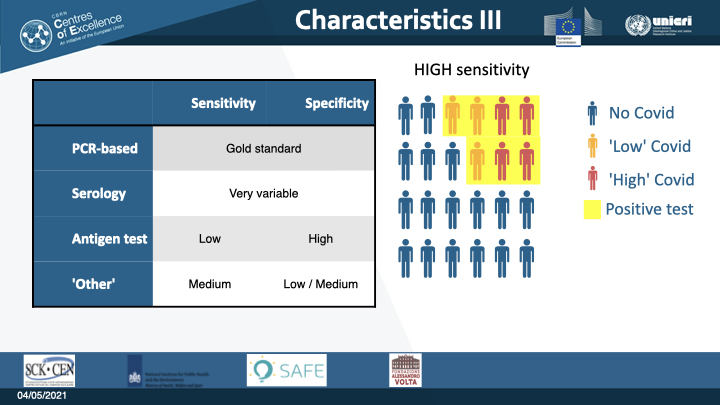
\includegraphics{images/m02/m02_types_of_rapid_tests_final.011.jpeg}

The PCR test performs very well in being
\RL{'}positive\RL{'} with persons carrying the virus.
Including the ones that are not sick. The test has excellent
sensitivity. There are hardly any false negative patients.

\begin{center}\rule{0.5\linewidth}{0.5pt}\end{center}

\textbf{Sheet 12 -- Characteristics IV}

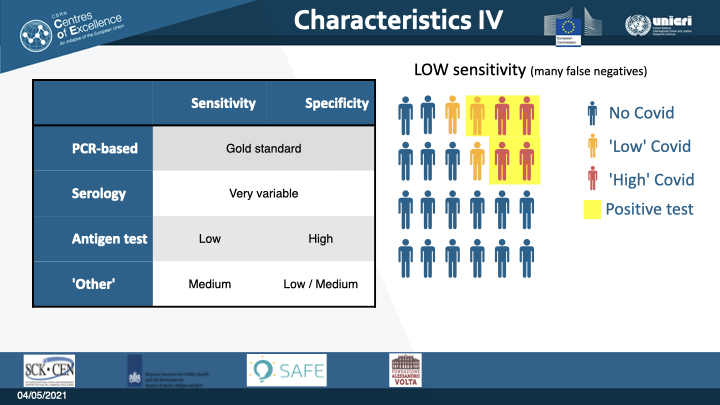
\includegraphics{images/m02/m02_types_of_rapid_tests_final.012.jpeg}

In another type of test, those persons that carry a low number of
viruses can be missed when the test has a low sensitivity. This type of
test is definitely not recommended in a setting with vulnerable persons,
for example in a maternity ward or an elderly home.

\begin{center}\rule{0.5\linewidth}{0.5pt}\end{center}

\textbf{Sheet 13 -- Characteristics V}

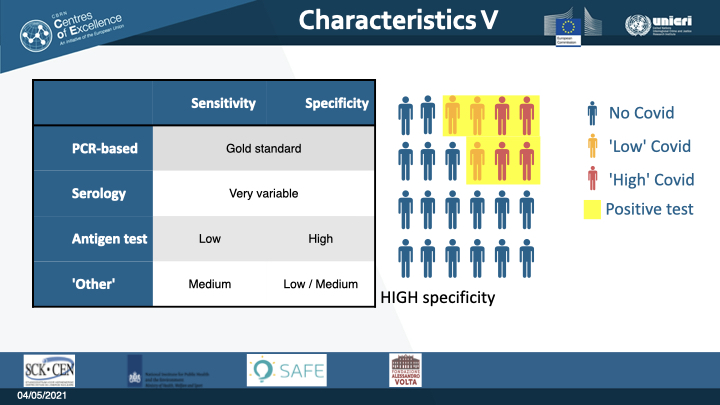
\includegraphics{images/m02/m02_types_of_rapid_tests_final.013.jpeg}

With the uninfected people, here, the test result is always
`\emph{negative}.' Hardly anyone gets a
false-positive result. The test has a great Specificity.

\begin{center}\rule{0.5\linewidth}{0.5pt}\end{center}

\textbf{Sheet 14 -- Characteristics VI}

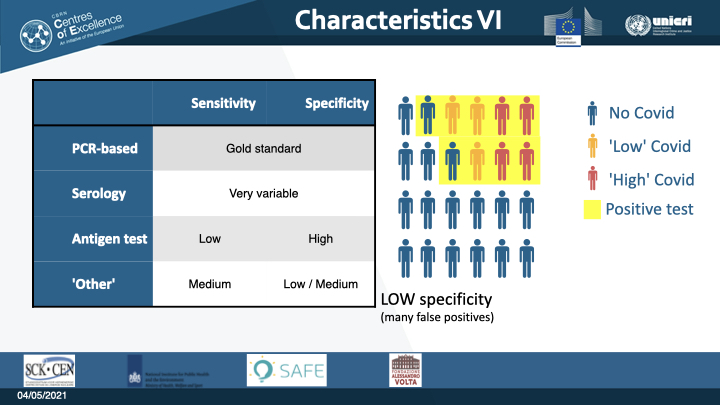
\includegraphics{images/m02/m02_types_of_rapid_tests_final.014.jpeg}

Low specificity comes when negative persons receive test result which
says they positive for the infection with the virus. Now, this does not
immediately mean that this test is useless. If this test is quick and
cheap, the `\emph{negative persons}' can carry on.
The positive ones, need to be double-checked with a more reliable test.
This, for example, would work in a setting for screening travellers.

For the sensitivity, it's always better to have it as high
as possible. But in some settings, one has to make a trade-off. Less
sensitivity for a faster and cheaper test. This is a complicated
decision.

\begin{center}\rule{0.5\linewidth}{0.5pt}\end{center}

\textbf{Sheet 15 -- Setting}

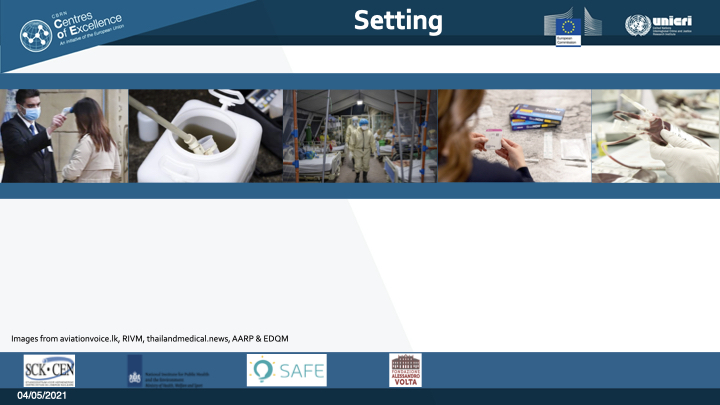
\includegraphics{images/m02/m02_types_of_rapid_tests_final.015.jpeg}

As showed, all types of tests have their advantages and disadvantages.
The first step before introducing a new test is to ask a few basic
questions:

For who is the test? Do we need to quickly screen passengers? Do we need
to diagnose a sick person? Do we need to monitor the environment or food
products?

What kind of samples are available? Throat or nose swabs? Feces?
Wastewater?

Where is the test conducted? At a laboratory? In a mobile health unit?
At home?

These questions are all part of formulating the objective when a new
test is to be validated.

\begin{center}\rule{0.5\linewidth}{0.5pt}\end{center}

\textbf{Sheet 16 -- Criteria}

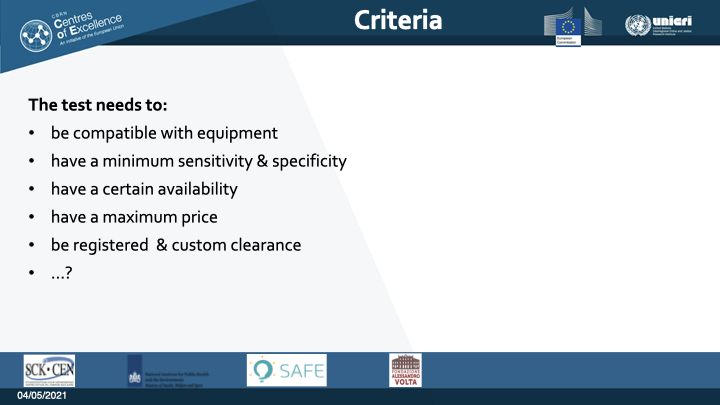
\includegraphics{images/m02/m02_types_of_rapid_tests_final.016.jpeg}

Once it is clear what the setting is, the list with tests can be further
shortened by setting several criteria. Do new reagents work with the
equipment already in the lab? What does the manufacturer state about the
sensitivity and specificity? And will the manufacturer be able to
provide enough test reagents for the near future? Also important is if
it is affordable? Are there any legal obligations before the test can be
purchased? Are the correct storage options available? This information
is all part of the validation plan.

\begin{center}\rule{0.5\linewidth}{0.5pt}\end{center}

\textbf{Sheet 17 -- Planning of Validation I}

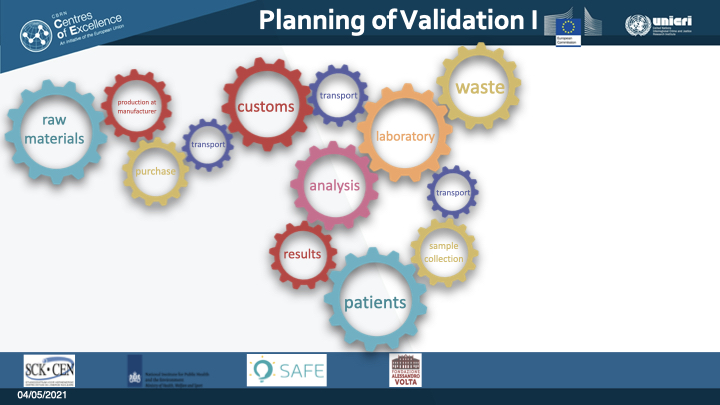
\includegraphics{images/m02/m02_types_of_rapid_tests_final.017.jpeg}

The reliability of a test does not only depend on the test itself. For
validating the test, processes associated with the collection and
production of the outcome needs investigation. It has to be confirmed
that all processes provide sufficient assurance that the results are
reliable. The validation also justifies why specific processes are
needed. Now, it is impossible to put all these processes into one
validation.

\begin{center}\rule{0.5\linewidth}{0.5pt}\end{center}

\textbf{Sheet 18 -- Planning of Validation II}

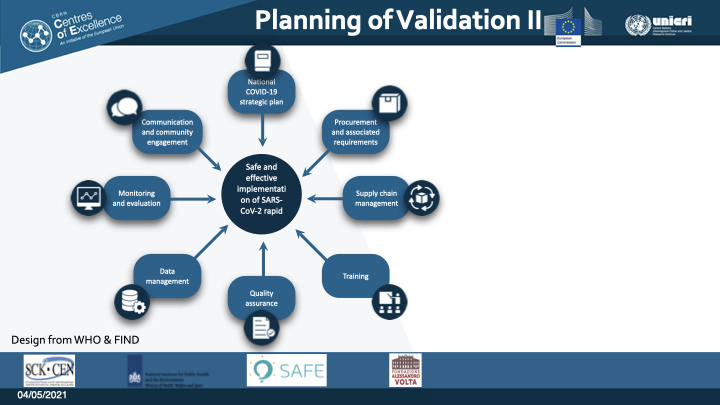
\includegraphics{images/m02/m02_types_of_rapid_tests_final.018.jpeg}

There are many actors involved in the successful implementation of a
test. For example, if storage at customs was inadequate, the reagent
might have deteriorated and can have a direct impact on the reliability
of the tests. The lab may validate as much as they can, the test results
remain unreliable. Therefore, it can be very rewarding to sit down with
relevant stakeholders and put yourself in their situation. It gives a
better understanding of all challenges. By facing the challenges
together, you might come up with an alternative for choosing the
appropriate test.

\begin{center}\rule{0.5\linewidth}{0.5pt}\end{center}

\textbf{Sheet 19 -- Summary}

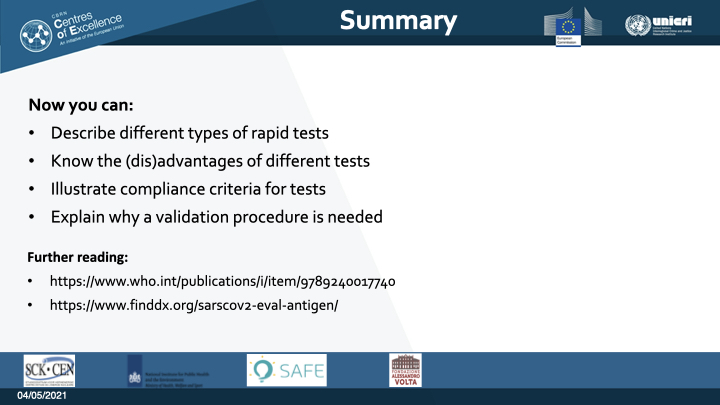
\includegraphics{images/m02/m02_types_of_rapid_tests_final.019.jpeg}

There was an overview of the types of tests that are being applied for
detecting SARS-CoV-2. It is made clear that one cannot just simply
compare one test with another. Especially when they are applied in
different settings.

\begin{center}\rule{0.5\linewidth}{0.5pt}\end{center}

\hypertarget{quiz-questions}{%
\subsection{Quiz questions}\label{quiz-questions}}

\hypertarget{faq}{%
\subsection{FAQ}\label{faq}}

\hypertarget{module-iii---validation-of-test-kits}{%
\section{Module III - Validation of test kits}\label{module-iii---validation-of-test-kits}}

\hypertarget{content-1}{%
\subsection{Content}\label{content-1}}

\begin{longtable}[]{@{}
  >{\raggedright\arraybackslash}p{(\columnwidth - 2\tabcolsep) * \real{0.25}}
  >{\raggedright\arraybackslash}p{(\columnwidth - 2\tabcolsep) * \real{0.74}}@{}}
\toprule
\endhead
\textbf{Length} & 14 minutes presentation \\
\textbf{Learning
goals} & The participants can:

\textbf{create} a validation report \\
\textbf{Summary} & \begin{minipage}[t]{\linewidth}\raggedright
Steps for validation of a rapid test are
explained.

\begin{itemize}
\item
  Rationale: why is this validation needed for?
  For example, conventional tests are expensive
  and shortage of consumables.
\item
  Objective: What is the primary (and secondary)
  question that needs to be answered? For
  example, what is the sensitivity?
\item
  Study population: Rapid tests are validated on
  well-defined user group. For example
  persons with Covid symptoms from
  the age of 16+, willing to
  participate, etc.
\item
  Methods: Ethical review, Statistics, primary \&
  secondary endpoints (use dummy graphics),
  procedure (questionnaire, sampling,
  type of tests, storage, transport, testing)
\item
  Main study endpoints: explain what will be
  measured? What is the reference standard?
\end{itemize}
\end{minipage} \\
\textbf{Tools \&
setup} & Ask participants to turn of (sound of) mobile
telephones

Explain if and when questions can be asked.

Relevant literature. PowerPoint slides. Presenter
in front of slides. Small quiz for recap. \\
\bottomrule
\end{longtable}

\hypertarget{narrative-1}{%
\subsection{Narrative}\label{narrative-1}}

\textbf{Sheet 03 - Training topics II}

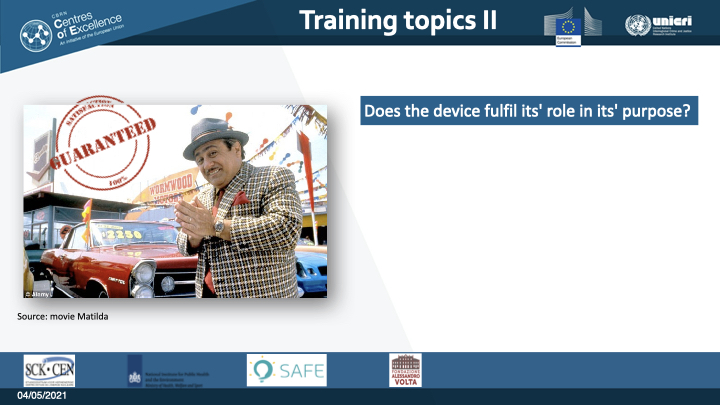
\includegraphics{images/m03/m03_validation_of_test_kits_v2_2.003.jpeg}

In the previous module, the main message about using new tests is that
one should not work blindly on promises of the manufacturer or
salesperson.

With a validation plan, we want to measure if the promises made by the
manufacturer meet real-life situations.

\begin{center}\rule{0.5\linewidth}{0.5pt}\end{center}

\textbf{Sheet 04 - Protocol synopsis}

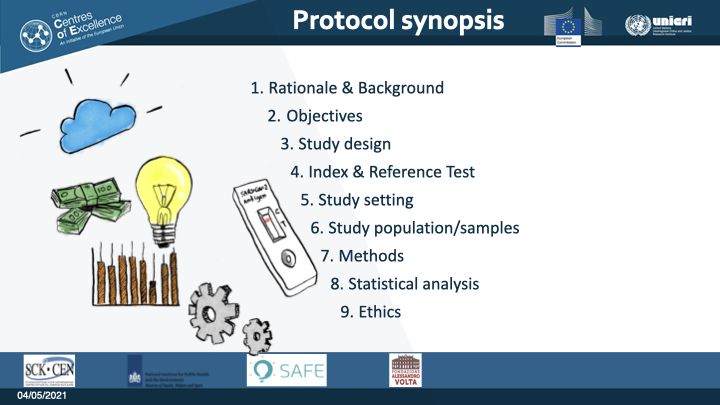
\includegraphics{images/m03/m03_validation_of_test_kits_v2_2.004.jpeg}

\textless p
These are the steps that will be briefly discussed. Of course, a plan
does not need to be limited to these chapters. The first chapter is
about explaining why the validation is carried out. The Objectives state
what exactly is going to be measured. The Study design is how the study
is set up. Chapter 4 explains which tests are going to be used. Chapter
six, who are the subjects and what type of samples are taken. In
methods, the procedures are explained in detail. For chapter eight i
will not explain the methods, but I\RL{'}ll illustrate the input
and output of data. Last but not least, the ethical aspects of the
study.

\begin{center}\rule{0.5\linewidth}{0.5pt}\end{center}

\textbf{Sheet 05 - 1. Rationale \& Background}

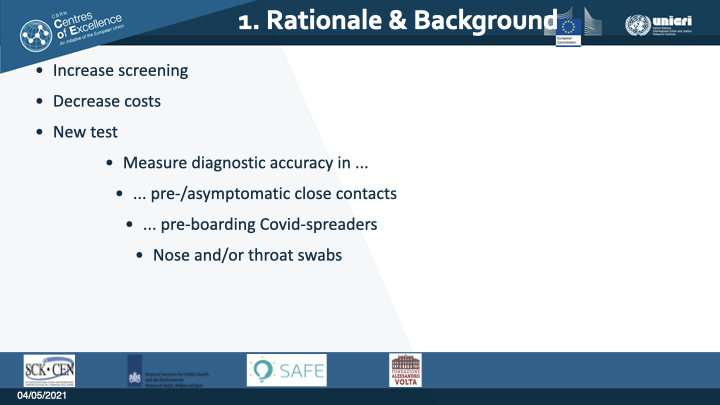
\includegraphics{images/m03/m03_validation_of_test_kits_v2_2.005.jpeg}

During the SARS-CoV-2 outbreak, the laboratory capacity quickly runs to
its limit and reagents were getting scarce. The time between getting a
patient sample until giving out the test result, also became an
important factor in the fight against Covid. Besides time, also costs
needed to go down. These are clear rationals to implement new rapid
tests: increase the speed of testing and decreasing costs. Once a
manufacturer or distributor of a new test is appointed, the test itself
should be verified. The manufacturer might promise 99\% sensitivity,
however, it might have been tested on sick hospital patients shedding
high loads of viruses. In your case, you might want to apply the test on
asymptomatic persons that had close contact with an infected person.
{[}PHOTO{]} Or, at the airport for pre-boarding Covid spreaders, you might
want to replace the body thermometer with a more sensitive breath
analyzer. {[}PHOTO{]} Validation can also be set up if a current process
needs to be adapted. For example to check if there is a difference in
sensitivity if one swab from the nasopharynx has the same sensitivity as
to when taking a double nasopharynx swab together with a throat-swab.
{[}PHOTO{]}

The rationale is to convince others why a change or investment in a new
method is needed.

\begin{center}\rule{0.5\linewidth}{0.5pt}\end{center}

\textbf{Sheet 06 - 2. Objectives I}

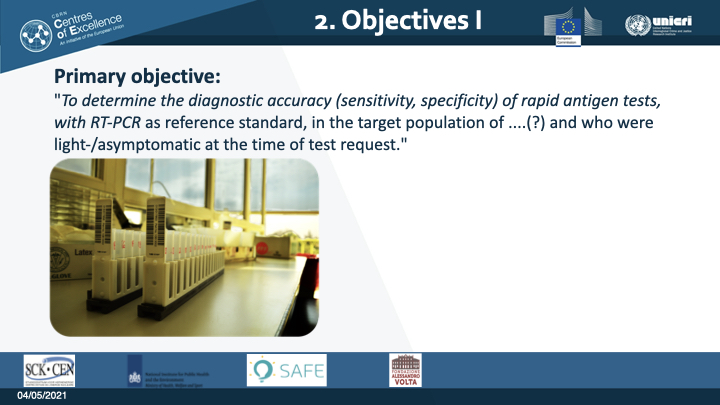
\includegraphics{images/m03/m03_validation_of_test_kits_v2_2.006.jpeg}

Suppose we want to check a new rapid test, the main objective is to
check the sensitivity and specificity of the test. How many false
positives and false negatives are detected with this new test? Here, it
needs to be clear who exactly the subjects are, and what kind of samples
are being used. It also needs to be clear what the reference method is.
The reference can be supplemented with more criteria, such as subjects
with specified clinical symptoms.

\begin{center}\rule{0.5\linewidth}{0.5pt}\end{center}

\textbf{Sheet 07 - 2. Objectives II}

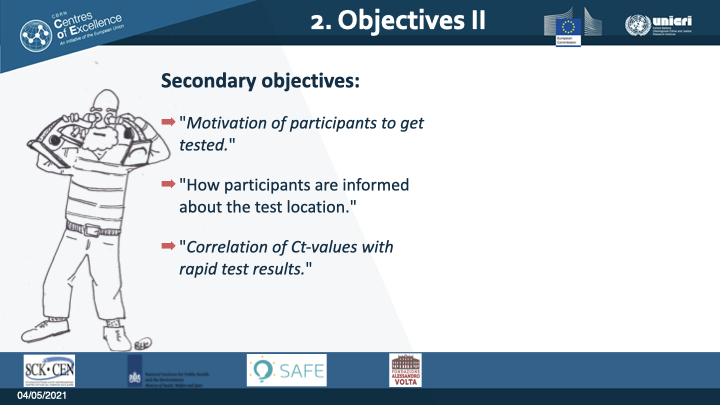
\includegraphics{images/m03/m03_validation_of_test_kits_v2_2.007.jpeg}

The experiment could be a good opportunity to gather more information,
besides the test itself. For example, a questionnaire could show that
many persons get tested is because they think they got infected with
SARS-CoV-2 from 5G radiation. In that case, a lot of resources could be
saved by starting an information campaign.

Correlation with Ct-values means if there is a pattern the positive and
negative outcome of the rapid tests, and the strength of the PCR
signals, which is expressed as Cycle-threshold values, or Ct values.

Hence, the objective of the plan is the research question, or the
hypothesis: what exactly do I want to measure or reproduce?

\begin{center}\rule{0.5\linewidth}{0.5pt}\end{center}

\textbf{Sheet 08 - 3. Study design}


\includegraphics{images/m03/m03_validation_of_test_kits_v2_2.008.jpeg}

The chapter on study design is a more technical explanation of how the
experiment is set up. In general, a test validation can be conducted in
a completely controlled environment in the laboratory. There is total
control over the parameters: samples were stored in the freezer and
concentrations of virus in the positive samples are well-defined. The
negative samples could be spiked with several respiratory viruses, other
than SARS-CoV-2, to check if the tests show cross-reaction with other
viruses. The test reagents are stored at the same temperature and the
equipment is handled by one researcher. The lab-based performance or
technical validation is usually already performed by the manufacturer.

In a clinical evaluation, there are many more uncertainties, a good
representation of real-life. Samples are taken from multiple sites, by
different persons, over a period of time, from unknown test subjects.
The study is blinded, which means that the technicians who are testing
the samples do not know if the samples are positive or negative. The
results are compared by an independent person.

\begin{center}\rule{0.5\linewidth}{0.5pt}\end{center}

\textbf{Sheet 09 - 4. Index \& Reference Test}

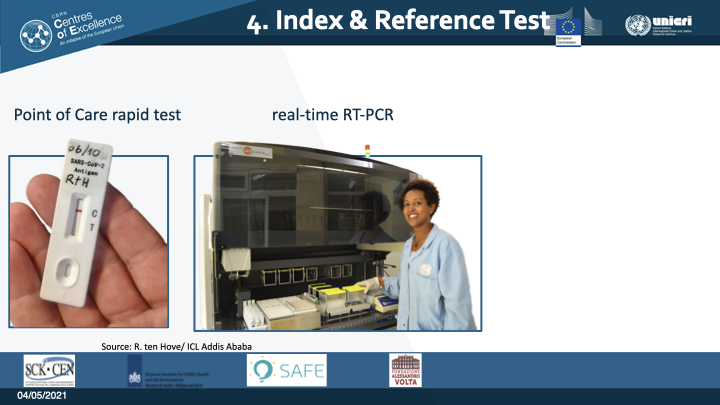
\includegraphics{images/m03/m03_validation_of_test_kits_v2_2.009.jpeg}

Index and reference test. In short, describe the test or maybe several
tests that need to be validated, and to what the method is being
compared to. It must be taken into account that, although PCR is
considered the gold standard, it is also not 100\% sensitive and
specific.

\begin{center}\rule{0.5\linewidth}{0.5pt}\end{center}

\textbf{Sheet 10 - 5. Study setting}

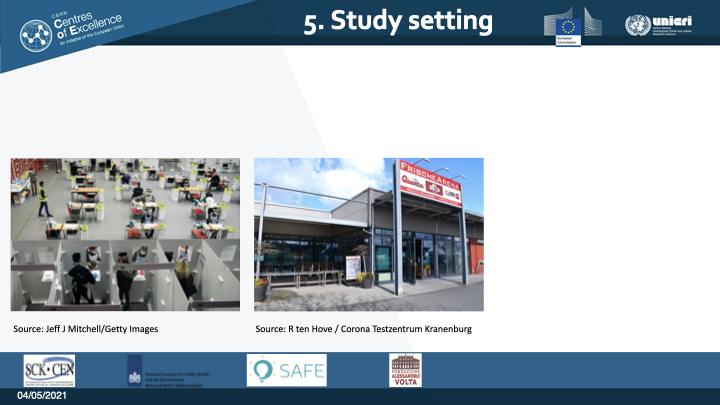
\includegraphics{images/m03/m03_validation_of_test_kits_v2_2.010.jpeg}

In this chapter, it is described where the samples are coming from. Are
the swab samples and data coming from one site or multiple sites? It
might be important when the demography of the subjects is described. A
testing centre at the university campus will provide samples from more
young persons, and thus likely to have samples with lower viral loads.

So, location can also be important for the interpretation of the
results.

\begin{center}\rule{0.5\linewidth}{0.5pt}\end{center}

\textbf{Sheet 11 - 6. Study population}

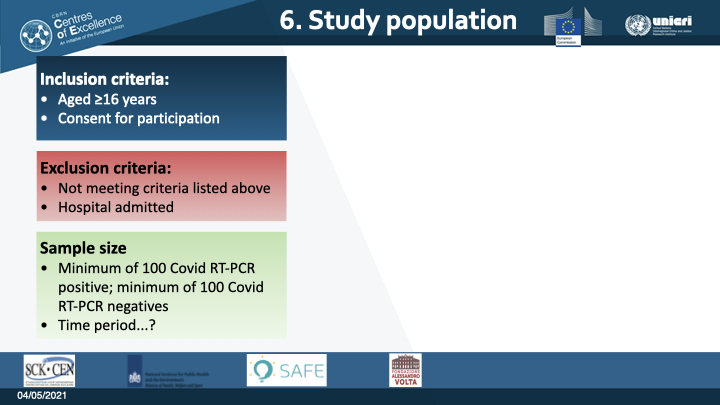
\includegraphics{images/m03/m03_validation_of_test_kits_v2_2.011.jpeg}

As mentioned in the previous sheet, age can be an important factor and
needs to be recorded to assure that the sample population is a
representative cross-section of the general population. The same applies
to gender. This chapter also needs to describe the inclusion criteria.
For example, children until 16 are excluded. Also, persons that are
mentally or physically unable to provide consent, should be excluded.
The test is validated for asymptomatic persons, therefore, subjects need
to be excluded from the study when they present Covid symptoms.
Basically, what is needed is a homogenous study population that
represents the study objective.

\begin{center}\rule{0.5\linewidth}{0.5pt}\end{center}

\textbf{Sheet 12 - 7. Methods}

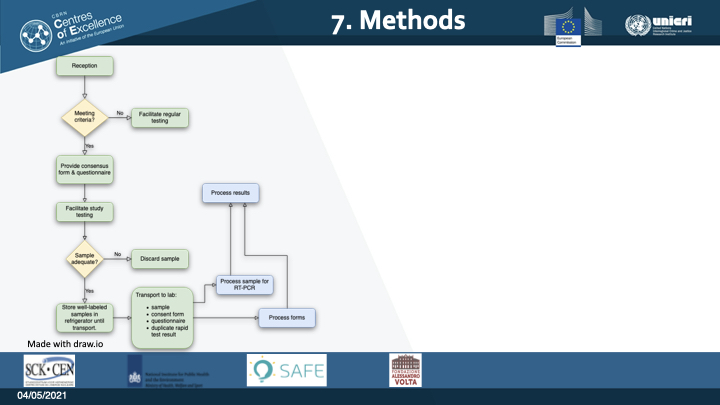
\includegraphics{images/m03/m03_validation_of_test_kits_v2_2.012.jpeg}

Here, a diagram shows all the steps during the study. It starts when the
subject presents itself at the reception, all the till the final
analysis of the test results. The chapter also describes the procedures,
among other how the swabs are taken and the PCR analysis. These
procedures can also be described in validated standard operation
procedures, which I will discuss in my next module. Different forms,
such as the questionnaire and the consent form can be added as an
appendix to the validation plan.

\begin{center}\rule{0.5\linewidth}{0.5pt}\end{center}

\textbf{Sheet 13 - 8. Statistical analysis I}

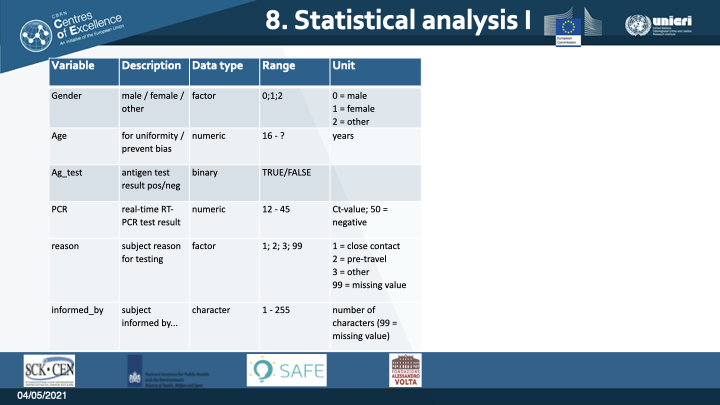
\includegraphics{images/m03/m03_validation_of_test_kits_v2_2.013.jpeg}

In this module I will not discuss the statistical methods: that would
take too long\ldots{} and boring for some. The important point here is that,
it would be very unfortunate if, at the end of the study, it appears
that conclusions cannot be made. Simply because we forgot to ask the age
of the subjects. How would we know for sure that we have an honest
representation of the general population? All work might have been done
for nothing.

Another tip is to structure all data. The most annoying thing for me as
a data scientist is to clean up data and use my own interpretation on
the collected data. For example, if the reason for testing says
``Family.'' What does that mean? Traveling to family? A
family member was Covid positive? Basically, if garbage data goes in,
garbage results come out.

\begin{center}\rule{0.5\linewidth}{0.5pt}\end{center}

\textbf{Sheet 14 - 8. Statistical analysis II}

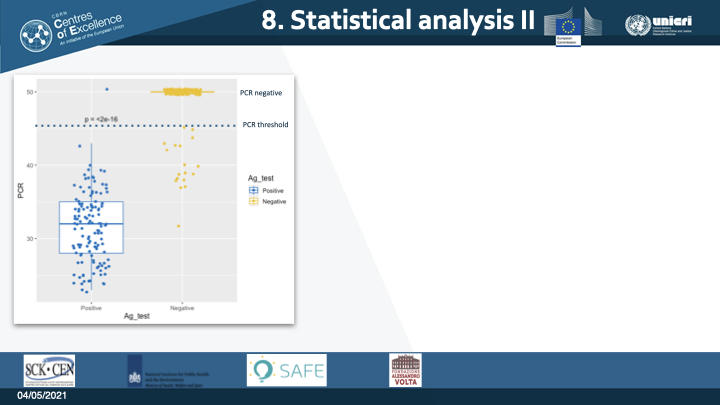
\includegraphics{images/m03/m03_validation_of_test_kits_v2_2.014.jpeg}

Here is an example of the statistical analysis. The numbers for this
graph are made up by the way. It's for illustration only.
At the bottom of the graph are the results of the rapid antigen test.
Blue dots on the left are antigen positive, and the yellow dots are
antigen negative. On the left side, it says PCR. Often the PCR results
are expressed in Ct-values. The lower the Ct-value, the stronger the
signal, meaning that there were many viruses in the samples. So, if the
Ct-value has a higher number, it means there were fewer viruses in the
sample. It goes up until it reaches a threshold. In this case, the
Threshold is value number 45. Above 45, there were no or too little
virus particles to be detected. For the data analysis, however, I gave
the PCR negative results the artificial Ct-value 50. All test results
with Ct value above 45\ldots{} or if no virus was detected, the sample gets
Ct value 50.

In the right column with yellow Antigen negative test results, you can
see that many of them still provided a positive PCR result. Most of them
were weak-positive, and have a high Ct-value. This is to be expected. In
the left column with blue Antigen positive test results, almost all of
them were also detected with PCR. There is, however, one exception. One
single blue dot above the threshold. The antigen was positive but the
PCR was negative. Maybe the PCR test went wrong. There was maybe an air
bubble in the reaction tube. Maybe the technician made an error and
swapped a sample? Still, I would not worry too much about it with these
results.

In any case, making some sketches of possible graphs and tables, before
the actual experiment starts, can help to improve the objective and
setup of the experiment.

\begin{center}\rule{0.5\linewidth}{0.5pt}\end{center}

\textbf{Sheet 15 - 9. Ethics}


\includegraphics{images/m03/m03_validation_of_test_kits_v2_2.015.jpeg}

For clinical experiments, consent of the participant is mandatory, at
least in most places. Consent is needed to use the samples and
information from the participants. But ask yourself: what information do
I need to reach my objectives? Do I really need the ethnicity of the
participant? Do I need to know their religion? What is the worst
case-scenario if all collected information would be stolen?

Another example, suppose the rapid test is negative. But later the PCR
shows to be positive. Do I need to inform the patient? A few things to
consider: if persons are to be informed, then private contact details
will have to be collected. Furthermore, if the PCR analysis is performed
two weeks later, is it then still worth tracing back the patient?

\begin{center}\rule{0.5\linewidth}{0.5pt}\end{center}

\textbf{Sheet 16 - Summary}

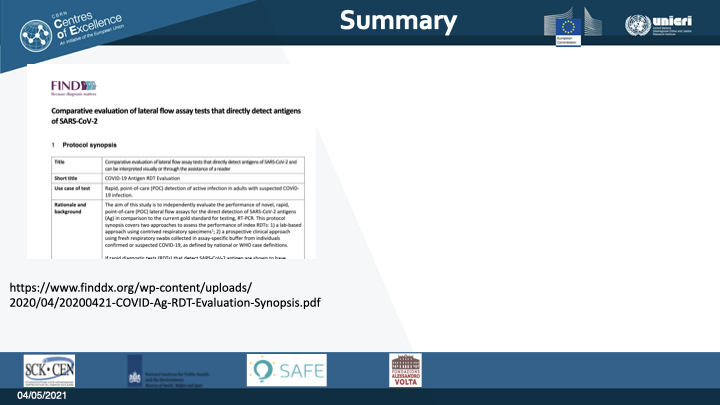
\includegraphics{images/m03/m03_validation_of_test_kits_v2_2.016.jpeg}

We went through every chapter of the validation plan. The most important
points are:

Describe the objective of the evaluation.

Make sure that the setup of the experiment is well thought through, and
does not need to be adapted halfway through, because we ran out of one
reagent. Therefore, it is important to involve all parties that play a
role in the validation. From finance to chauffeur.

Also, statisticians, they can fix mistakes, but only to a certain level.
Better to involve them in the set-up.

And last but not least, the ethics involved with the validation.

\begin{center}\rule{0.5\linewidth}{0.5pt}\end{center}

\hypertarget{quiz-questions-1}{%
\subsection{Quiz questions}\label{quiz-questions-1}}

\hypertarget{faq-1}{%
\subsection{FAQ}\label{faq-1}}

\hypertarget{module-iv---quality-management}{%
\section{Module IV - Quality Management}\label{module-iv---quality-management}}

\hypertarget{content-2}{%
\subsection{Content}\label{content-2}}

\begin{longtable}[]{@{}
  >{\raggedright\arraybackslash}p{(\columnwidth - 2\tabcolsep) * \real{0.25}}
  >{\raggedright\arraybackslash}p{(\columnwidth - 2\tabcolsep) * \real{0.74}}@{}}
\toprule
\endhead
\textbf{Length} & 12 minutes presentation \\
\textbf{Learning
goals} & \begin{minipage}[t]{\linewidth}\raggedright
The participants can:

\begin{itemize}
\item
  \textbf{Argue} the need of standard procedures.
\item
  \textbf{Judge} if a batch can be released.
\item
  \textbf{Evaluate} potential risks during the
  testing procedures.
\end{itemize}
\end{minipage} \\
\textbf{Summary} & \begin{minipage}[t]{\linewidth}\raggedright
Topics of the module include:

\begin{itemize}
\item
  What is Quality Management and why do we need
  it?
\item
  Why do we need Standard Operation Procedures?(
  for example for using the rapid test)
\item
  Batch release.
\item
  Risk assessment.
\end{itemize}
\end{minipage} \\
\textbf{Tools \&
setup} & Ask participants to turn of (sound of) mobile
telephones

Explain if and when questions can be asked.

Relevant literature. PowerPoint slides. Presenter
in front of slides. Small quiz for recap. \\
\bottomrule
\end{longtable}

\hypertarget{narrative-2}{%
\subsection{Narrative}\label{narrative-2}}

\textbf{Sheet 03 - Learning objectives}

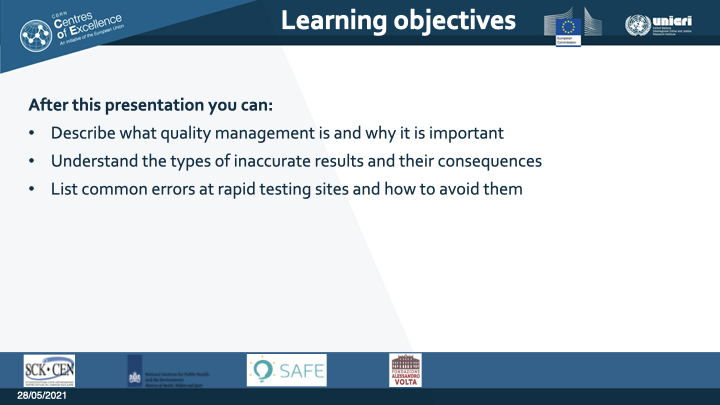
\includegraphics{images/m04/m04_Quality_management_v3.003.jpeg}

First of all, the terms SARS-CoV-2 and COVID may be used
interchangeably. SARS-CoV-2 is the correct term for the virus, but I
will sometimes abbreviate it simply as Covid.

Second, the focus is mainly on Quality Management for settings where
rapid antigen tests are used. Still, the information can also be applied
for other settings.

Now, about Quality management. This term might be considered as some
upper level vague concept. In reality, quality management affects every
single step and procedure inside and outside the laboratory. From
receiving the patient or client, to submitting the test result. Any weak
link or error in the course of actions could set in a chain reaction
with disastrous effects in the end. It can be something small as not
monitoring the temperature of the refrigerator, or getting sloppy with
personal protection. I will discuss these types of risks, their
consequences and how to avoid them.

\begin{center}\rule{0.5\linewidth}{0.5pt}\end{center}

\textbf{Sheet 04 - QC/QA/QM}

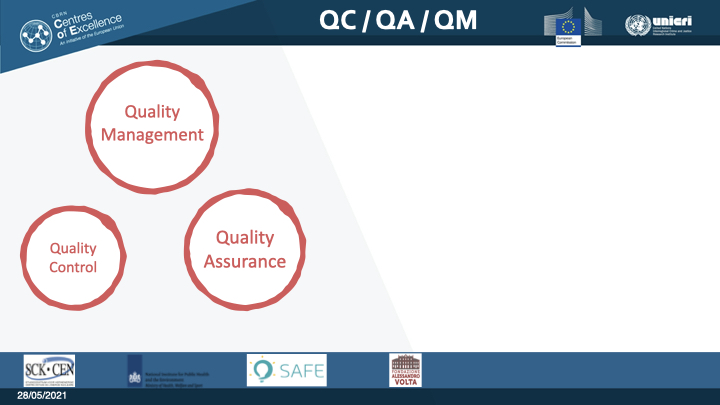
\includegraphics{images/m04/m04_Quality_management_v3.004.jpeg}

Quality control, quality assurance and quality management, these terms
might be confusing. In general, they can be described as follows.

\begin{center}\rule{0.5\linewidth}{0.5pt}\end{center}

\textbf{Sheet 05 - Quality Control I}

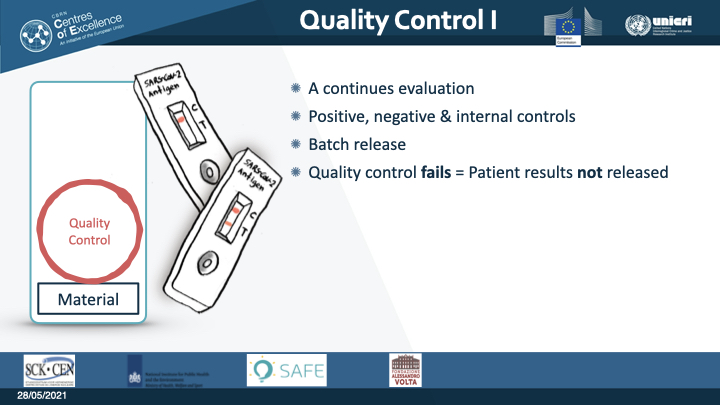
\includegraphics{images/m04/m04_Quality_management_v3.005.jpeg}

Quality control involves the continuous evaluation or monitoring of the
performance of the Covid Antigen Rapid diagnostic tests. This is to
ensure that all steps are correctly followed, steps that are required
for accurate diagnosis.

Quality control consists of samples with from which it is known they are
POSITIVE or NEGATIVE.

These reference samples are used regularly in accordance with the
manufacturer's instructions and national policy. It is advisable to
perform QC testing at least once a week or more frequently if the
testing site has conducted a high number of tests.

Another moment to perform a Quality control test is when a new batch or
lot number of Antigen rapid tests is going to be deployed. At least five
samples (three positive and two negative) should be tested for each new
lot. One could add rapid tests both from the ones currently in use, and
from the new lot number

Quality control fluids may be supplied with the Covid Antigen test kit.
If materials are not supplied with the kit, they can be purchased kit
supplier or a third-party provider. Another method is to pool positive
and negative patient material. If the quality control results do not
match the expected results, Quality control has failed. Investigation
and corrective actions are required.

\textbf{Patient test results cannot be released if quality control fails.}

\begin{center}\rule{0.5\linewidth}{0.5pt}\end{center}

\textbf{Sheet 06 - Quality Control II}

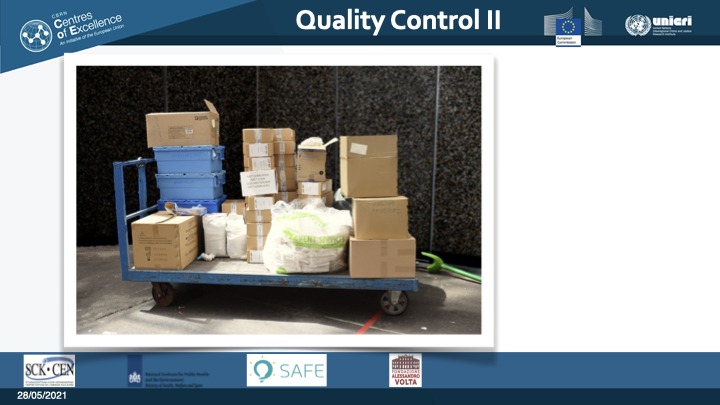
\includegraphics{images/m04/m04_Quality_management_v3.006.jpeg}

Quality control for the release of new batches does not only apply for
the rapid tests. It applies for all consumables, including the swabs,
the masks, the disinfection fluid. New material and batches need to be
checked and evaluated if they meet the specified requirements.

This is a picture made at a testing site. The wagon containing material
that do not pass the quality control. For example these swabs.. \emph{{[}Show
swabs that did not pass QC{]}}

\begin{center}\rule{0.5\linewidth}{0.5pt}\end{center}

\textbf{Sheet 07 - Quality Assurance}

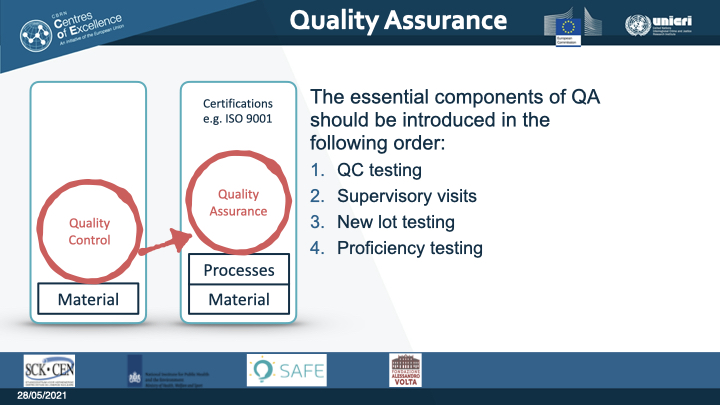
\includegraphics{images/m04/m04_Quality_management_v3.007.jpeg}

The next level concerns quality assurance. Even if all material passed
their quality control test, if they are used in a wrong matter, the
patient can still be sent out with the false result.

Given the need to quickly roll out COVID Antigen Rapid testing, a full
Quality Assurance system may not be in place when testing is started.
Therefore, to maximize quality, it is essential that a good-quality
Rapid Diagnostic Test product is purchased, and then transported and
stored according to the manufacturer's instructions. The
users must be trained and supervised, but with a mechanism in place for
them to report concerns and complaints.

The essential components of Quality assurance should be introduced in
the following order:

1. QC testing
2. Supervisory visits or audits
3. New lot testing, or new lot verification of incoming kits
4. Proficiency testing

\begin{center}\rule{0.5\linewidth}{0.5pt}\end{center}

\textbf{Sheet 08 - Quality Management}

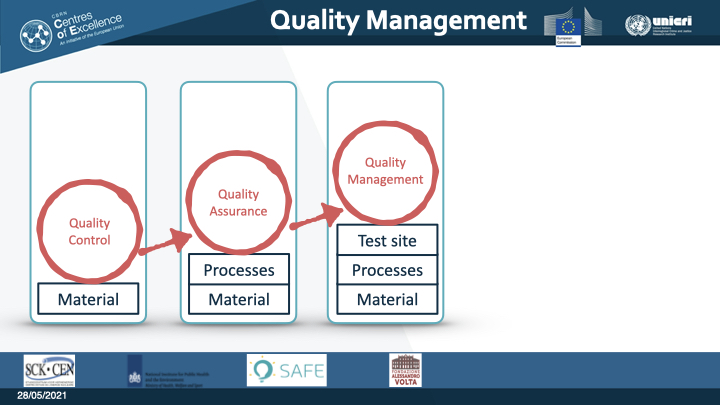
\includegraphics{images/m04/m04_Quality_management_v3.008.jpeg}

Quality assurance requires a lot of organization. The personnel on the
ground do not have time for this. Also they might be biased. Quality
management usually in the hands of a dedicated Quality Manager. The
manager does not necessarily need to have a technical background, and
knows all the in's and out's of the laboratory. The role of the
quality manager is to assure that procedures are kept in place. The
manager organised the internal audits. The manager receives any incident
reports and makes sure they are being followed up.

In short, quality control is about materials, quality assurance how
materials are being used, and quality management how everything is
organized.

\begin{center}\rule{0.5\linewidth}{0.5pt}\end{center}

\textbf{Sheet 09 - EQA}

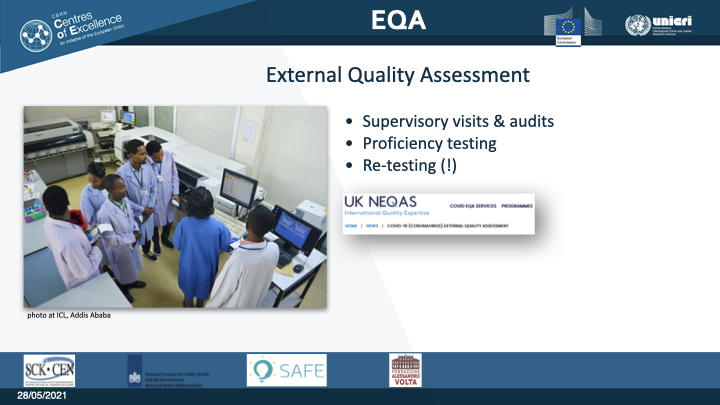
\includegraphics{images/m04/m04_Quality_management_v3.009.jpeg}

There are a few more elements regarding Quality Assurance, which are
grouped as External Quality Assurance.

Before the testing site is opening its doors, a supervisory visit can
assess the readiness of the place. On the website of this module you can
download an example of a testing site readiness checklist.

After the testing has started, the site can be assessed periodically,
for example four times per year. Or more often when there are frequently
problems recorded. You can also download the testing site supervisory
checklist.

A proficiency testing program can be used to identify and resolve
problems in diagnostic testing. Well characterized samples can be used
for proficiency testing. The sample could for example contain different
loads of the virus. Samples can be purchased from external agencies, for
example NEQAS. Samples can also be exchanged between testing sites.

For Quality Assurance, patient samples could also be retested at a
different site. However, this is not advisable due to the practicality
of collecting multiple samples and the safety associated with their
transport.

\begin{center}\rule{0.5\linewidth}{0.5pt}\end{center}

\textbf{Sheet 10 - Root cause analysis}

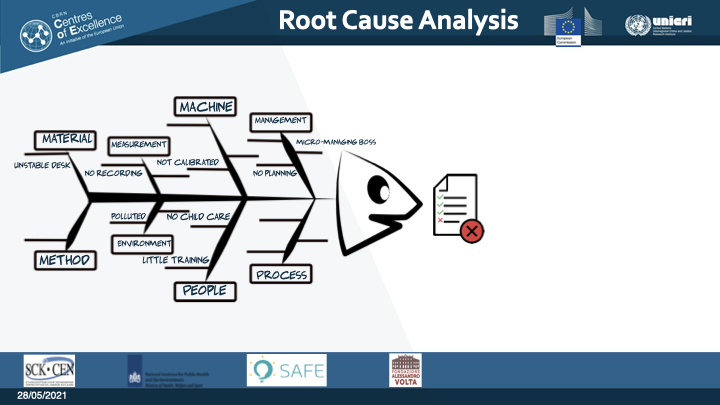
\includegraphics{images/m04/m04_Quality_management_v3.010.jpeg}

Failed proficiency test, or any other major mistake, requires
investigation. The reason for the error need to be uncovered. This is
called root cause analysis. An example of a tool is this fish bone
method, where different areas are systematically examined. When the root
cause has been identified, corrective action must take place.
Furthermore, preventive actions should prevent the reoccurrence of the
mistake. These errors and actions must be documented by the testing
site.

\begin{center}\rule{0.5\linewidth}{0.5pt}\end{center}

\textbf{Sheet 11 -When do errors occur? - I}

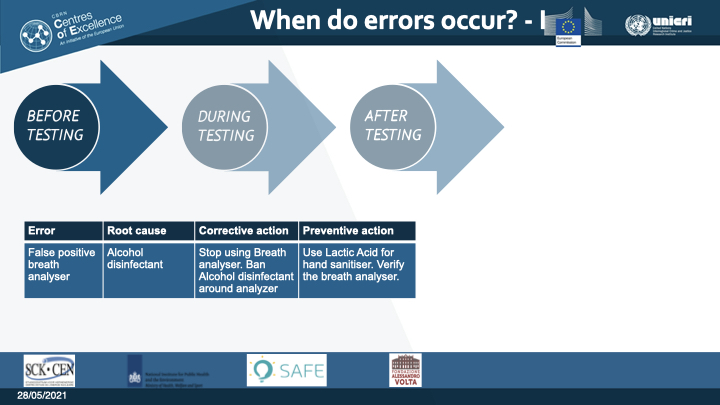
\includegraphics{images/m04/m04_Quality_management_v3.011.jpeg}

Before entering the testing site, clients need to sanitize their hand
with alcohol dispenser. They are first directed to the breath analyzer.
If the analyzer is negative, the client is safe and can go out. If the
analyzer result is 'undetermined', the client needs to do a rapid PCR
or LAMP test. However, it quickly becomes clear there is something wrong
with the analyses. At the end of the day, almost all clients test
results become undetermined.

The root cause is the alcohol hand sanitizer. The breath analyzer is too
sensitive. The corrective action is to stop using the breath analyzer
and direct all clients to the LAMP test. The preventive action is to
introduce lactic acid and ban all alcohol disinfectants around the
breath analyzer. With the new preventive action, samples are run in
parallel both with the breath analyser and the LAMP test.

\begin{center}\rule{0.5\linewidth}{0.5pt}\end{center}

\textbf{Sheet 12 -When do errors occur? - II}

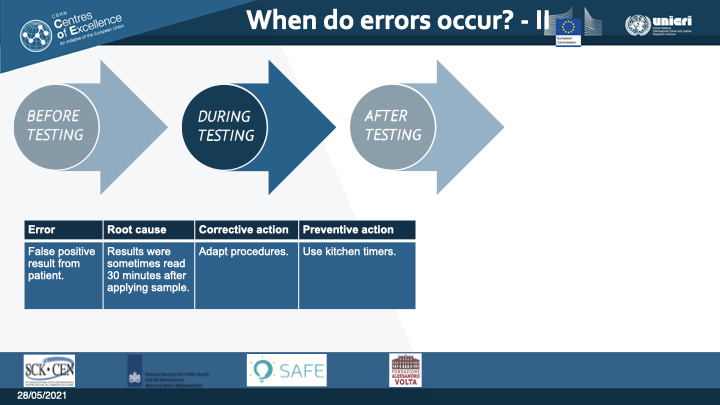
\includegraphics{images/m04/m04_Quality_management_v3.012.jpeg}

In another setting where rapid antigen tests are used. It's very
convenient as test results are provided on the spot. The number of
patients grow quickly, and then the weekly reports show that the
percentage of positive patients is increasing significantly, from 12 \%
to 45\%. An increasing number of patients complained that they had to go
into quarantine, but never tested positive in the following days. The
root cause analysis showed that when there are a lot of customers, the
technicians sometimes failed to check the results after 15 minutes.
Sometimes the results were checked after 30 minutes. Antigen can become
false positive when they are left too long. A solution was to buy the
manual kitchen timers and put is with each rapid test. Also, when it
becomes busy, the floor manager is helping in the process.

\begin{center}\rule{0.5\linewidth}{0.5pt}\end{center}

\textbf{Sheet 13 -When do errors occur? - III}

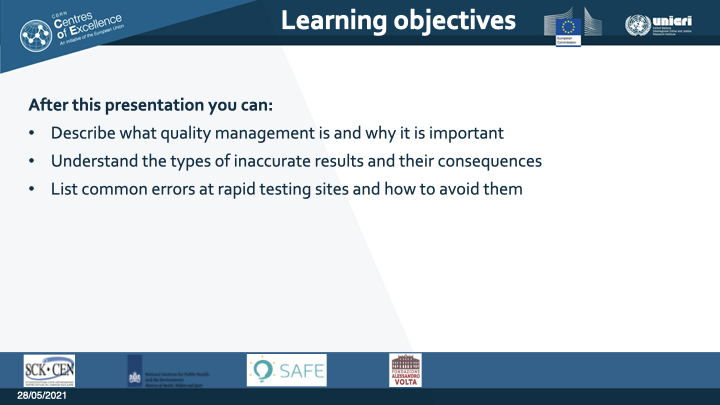
\includegraphics{images/m04/m04_Quality_management_v3.003.jpeg}

After the testing is done, the test results are shared with the
customers. The next day, however, it became clear that the results of
two patients with the same name were swapped. One was false positive and
went into quarantine. Also, also the close contacts also went for Covid
testing. The other person who was tested false negative, became ill the
next day. After giving sincere apologies, the close contacts of the
Covid patient had to be traced. Clearly, using the patient name as a
single identifier is not enough.

\begin{center}\rule{0.5\linewidth}{0.5pt}\end{center}

\textbf{Sheet 14 -Summary}

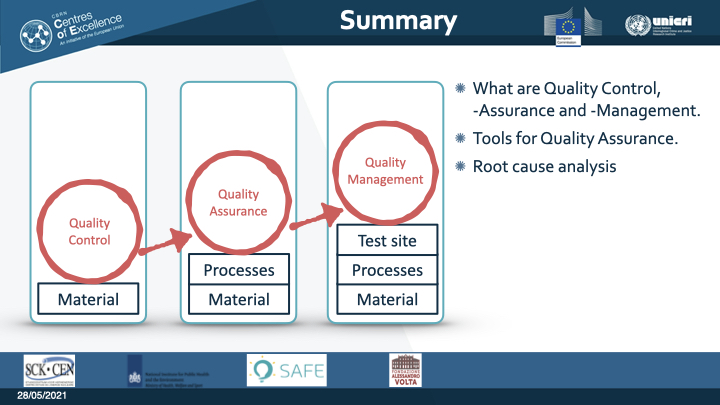
\includegraphics{images/m04/m04_Quality_management_v3.014.jpeg}

In this presentation it was explained what quality control, assurance
and management are. Several tools and examples were shown on how to
implement quality assurance at a testing site. One of the tools is root
cause analysis, for the continues improvement of the testing facility.

\begin{center}\rule{0.5\linewidth}{0.5pt}\end{center}

\hypertarget{quiz-questions-2}{%
\subsection{Quiz questions}\label{quiz-questions-2}}

\hypertarget{faq-2}{%
\subsection{FAQ}\label{faq-2}}

\hypertarget{module-v---workflow}{%
\section{Module V - Workflow}\label{module-v---workflow}}

\hypertarget{content-3}{%
\subsection{Content}\label{content-3}}

\begin{longtable}[]{@{}
  >{\raggedright\arraybackslash}p{(\columnwidth - 2\tabcolsep) * \real{0.25}}
  >{\raggedright\arraybackslash}p{(\columnwidth - 2\tabcolsep) * \real{0.74}}@{}}
\toprule
\endhead
\textbf{Length} & 15 minutes \\
\textbf{Learning
goals} & The participants can:

\textbf{Design} a proper and safe workflow in a routine
testing facility. \\
\textbf{Summary} & Proper registration procedures are explained to
avoid mis-diagnosis. Biosafety work procedures for
the protection of staff, clients and environment,
which also include safe discard of waste. Examples
of crowd control methods are shown to improve the
testing-flow and a safe environment for the
clients and staff. \\
\textbf{Tools \&
setup} & Ask participants to turn of (sound of) mobile
telephones

Explain if and when questions can be asked.

Relevant literature. PowerPoint slides. Presenter
in front of slides. Small quiz for recap. \\
\bottomrule
\end{longtable}

\hypertarget{narrative-3}{%
\subsection{Narrative}\label{narrative-3}}

\textbf{Sheet 03 - Learning Objectives}

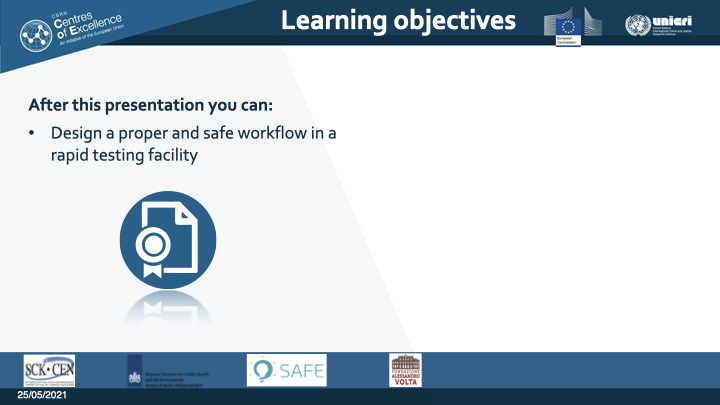
\includegraphics{images/m05/m05_Workflow_final.003.jpeg}

After this presentation, you will be familiar with the design of a
proper and safe workflow in a rapid testing center. Safe for both the
clients and the staff. Not all details can be covered in a quarter of an
hour. Still, hoping that by showing some examples, it will inspire you
and you will come up with new ideas and solutions to improve the testing
facility.

\begin{center}\rule{0.5\linewidth}{0.5pt}\end{center}

\textbf{Sheet 04 - Testing center area}

\begin{figure}
\centering
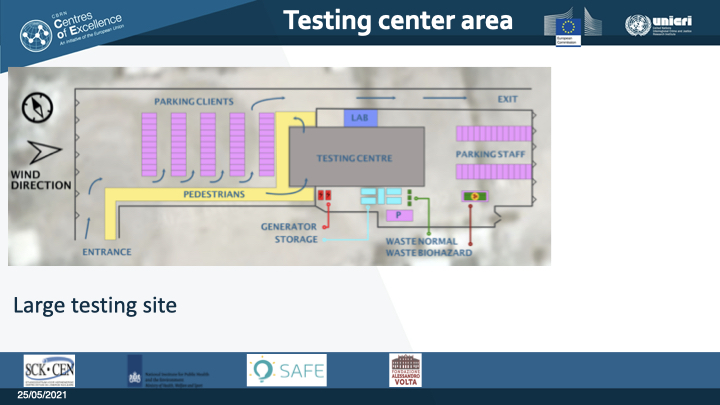
\includegraphics{images/m05/m05_Workflow_final.004.jpeg}
\caption{sheet 04}
\end{figure}

When a large new testing center is set-up, it might be naturally to fit
it with existing facilities, for example in a hospital. However, the
large influx of visitors can cause problems, for example from traffic
jams and large crowds.

Is is therefor recommended for the testing area to set up in places that
can be easily reached and has plenty of parking space. On the sketch the
testing center is in between two areas. One for the clients and the
other for staff. The areas can be separated by fences. Traffic
controllers check at the entrance if visitors come for testing, and not
because they want to park their car and go shopping at the nearby mall.
The traffic controllers can also help prevent that the testing center
gets overcrowded. Other things to consider when the testing site is set
up, are canals to drain excess of water during heavy rain, or damage
from heavy winds. Here is a picture of a testing-site in The Netherlands
{[}PHOTO\_04\_1{]} . The entrance and exit are clearly marked. Also the
Emergency exits need to be clearly visible. {[}PHOTO\_04\_2{]}

Some visitors may be handicapped or are less mobile. A dedicated parking
space for immobile clients close to the entrance might be helpful.

Some of the waste should be considered as biohazard. {[}PHOTO\_04\_3{]}. The
waste can be disclosed from the public and marked with a biohazard sign.

\begin{center}\rule{0.5\linewidth}{0.5pt}\end{center}

\textbf{Sheet 05 - Small test center}

\begin{figure}
\centering
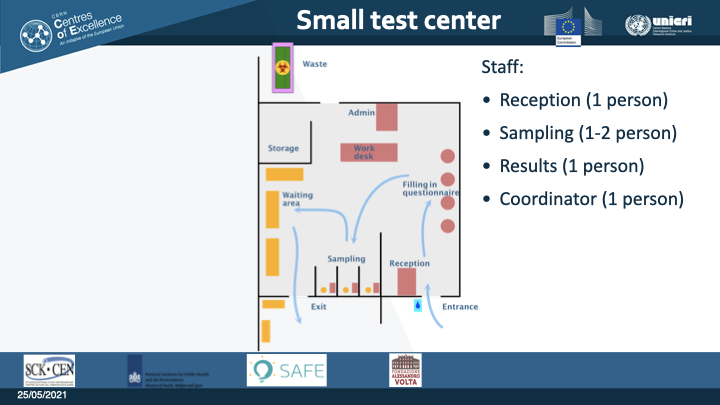
\includegraphics{images/m05/m05_Workflow_final.005.jpeg}
\caption{sheet 05}
\end{figure}

Here is a sketch from a small test centers. These can be opened up at
any location. It can even be a transformed cafeteria {[}PHOTO\_05\_1{]} or a
camping van {[}PHOTO\_05\_2{]}.

On the lay-out you can see that the clients all follow one direction. At
the entrance the host asks if the client has specific symptoms and can
check the temperature. The client receives a questionnaire
{[}PHOTO\_5\_3{]}, which might be translated into different languages. The
clients can fill in the questionnaire separately at a table. Next, they
hand over the paper to the sample taker. {[}PHOTO\_05\_4; PHOTO\_05\_5{]} .
Another staff member receives the samples together with the client
forms. This person makes sure that the results are read at 15 minutes,
for example by using these cooking clocks {[}PHOTO\_05\_6{]}

The testing site can have an additional person who is responsible for
the inventory and jumps in when extra help in needed. Furthermore, there
should be a clear protocol for certain situations. What if the client
has COVID-symptoms? What should be done when a test result is positive?
What should be done when the quality control of the test fails? This is
all part of the Quality Management of the site, which was discussed in
the previous module.

\begin{center}\rule{0.5\linewidth}{0.5pt}\end{center}

\textbf{Sheet 06 - Large test center I}

\begin{figure}
\centering
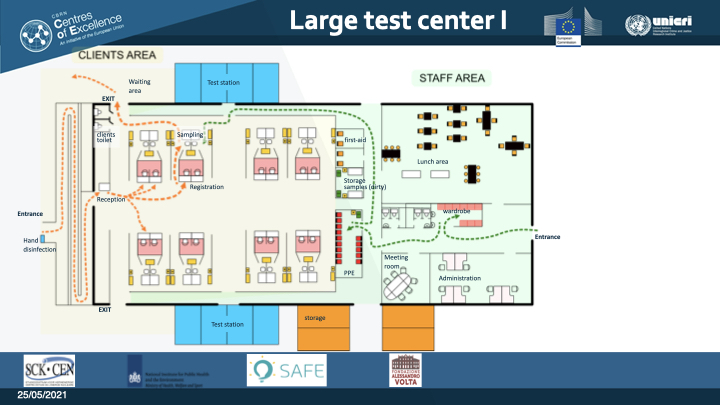
\includegraphics{images/m05/m05_Workflow_final.006.jpeg}
\caption{sheet 06}
\end{figure}

Here, the lay-out of a large testing facility is drawn. The yellow part
is the dedicated Clients area. The green part is the area for the staff
and where clients are not allowed. Behind the testing-booths, there is a
separate corridor. The staff can reach the testing booths from behind,
and they don't have to cross the area with the clients. In the next
slide I will go step by step at each location inside the testing center.

\begin{center}\rule{0.5\linewidth}{0.5pt}\end{center}

\textbf{Sheet 07 - Large test center II}

\begin{figure}
\centering
\includegraphics{images/m05/m05_Workflow_final.007.jpeg}
\caption{sheet 07}
\end{figure}

First the clients area. All the way at the left is the entrance, still
outside the center. The client disinfects the hands and walks down the
aisle. As you can see, the client has to make this detour to reach the
reception. The detour takes around 30 seconds, exactly the time needed
for the hand-disinfectant to do its job. The host at the reception can
do the first intake. For example, to check if the clients has their
identification with them. The host can provide instructions to go to an
available booth. {[}PHOTO\_07\_1{]} If it concerns a child for example, they
can be directed to a special booth that is arranged specially for
children. Or direct someone to a booth that is accessible for their
wheelchair. {[}PHOTO\_07\_2{]} The booths can have red or green light or
monitor screens to indicate if the booth or lane is available.

Here is a photo of the registration counter. {[}PHOTO\_07\_3{]} There is
glass in between. On the glass there is clearly indicated that the
ID-card can be presented in the square on the glass. This to prevent
that clients push their papers directly under the glass. Next, the
client moves to sampling spot behind the booth. Here, attention should
be paid that there is no mismatch between the client, and the
information on the test-tube. There can be for example a centralized
computer system where a sticker with a bar-code comes out of a label
printer at the sampling spot. {[}PHOTO\_07\_4{]} Still, the person taking
the sample should always double check if the information on the
test-tube matches the information from the client.

When sampling is done, the client is directed to the exit.
{[}PHOTO\_07\_5{]} Colored lines on the floor can help the client to reach
the nearest exit. Outside, the client can wait for the test result.

\begin{center}\rule{0.5\linewidth}{0.5pt}\end{center}

\textbf{Sheet 08 - Large test center III}

\begin{figure}
\centering
\includegraphics{images/m05/m05_Workflow_final.008.jpeg}
\caption{sheet 08}
\end{figure}

Now we enter the testing facility from the staff entrance. The personnel
can lock their properties in in the wardrobe. In the lunch area, before
the shift starts, the personnel gets the latest updates and their
work-sheets. After a coffee, the staff goes to the room where they put
on their personal protective equipment or PPE. {[}PHOTO 08\_1 \& 08\_2{]}.
The tables should be clearly labeled that they are clean. Meaning, no
used PPE are allowed on or around the table. This can also be
highlighted with green and red tape.

For large testing sites, basic walkie talkies can be used {[}PHOTO\_08\_3{]}
to stay in contact with colleagues, without the need of walking around
with potential contaminated dressing and equipment, or shouting for
assistance. Here is a pictures of two lanes separated with a wall
{[}PHOTO\_08\_4{]}. The lane on the right is for staff. The left lane is for
clients, with the blue line on the floor that directs them to the exit.

The staff member walks through the staff-corridor to their booth
{[}PHOTO\_08\_5{]}. At the booth, the administrator takes seat behind the
desk. If the place is well ventilated, he or she does not need full PPE.
However, proper distance should be kept from from the colleague behind
who is taking swabs from clients.

The person taking swabs makes sure that there is plenty of material.
{[}PHOTO\_08\_06{]} before he or she starts the shift.

The tubes with the swabs can be collected and moved to the test station.
There, they are tested with the Ag rapid tests or rapid PCR tests.
{[}PHOTO\_08\_7{]} This picture is taken from a PCR laboratory, which needs
an air-confined containment. Here, the samples are passed to the
air-controlled laboratory through a lock with two windows. This strict
air-containment is not needed when Antigen or serology tests are
performed. If samples need to be send to a different location, they can
then be stored in a refrigerator. {[}PHOTO\_08\_8{]} These can be for
example samples collected for additional genotyping analysis for
monitoring SARS-CoV-2 strains.

\begin{center}\rule{0.5\linewidth}{0.5pt}\end{center}

\textbf{Sheet 09 - Large test center IV}

\begin{figure}
\centering
\includegraphics{images/m05/m05_Workflow_final.009.jpeg}
\caption{sheet 09}
\end{figure}

Basically, at the test-center we need personnel for administration, we
have a person taking the samples, a person collecting all the samples
and moving them to the test station. We have someone dedicated to fill
up the inventory. If a problem occurs on the floor, for example a
mismatch with someones identification, a floor manager can jump in and
provide assistance. Occasionally it can happen that someone gets a
bleeding nose, or that someone faints. These clients can be helped in
the first-aid room by someone who is trained for this.

\begin{center}\rule{0.5\linewidth}{0.5pt}\end{center}

\textbf{Sheet 10 - Drive through}

\begin{figure}
\centering
\includegraphics{images/m05/m05_Workflow_final.010.jpeg}
\caption{sheet 10}
\end{figure}

These are picture of a drive through testing site. It is the same
principle, although clients do not get their test-result in person, but
receive them by email or on an app. At the entrance the host directs the
client to an available lane. Engines should be turned of when the care
is standing still to protect staff from car-fumes. There is a parking
spot at the back if, for example there an administrative or medical
problem, and assistance is needed from the floor manager.

\begin{center}\rule{0.5\linewidth}{0.5pt}\end{center}

\textbf{Sheet 11 - Training of staff}

\begin{figure}
\centering
\includegraphics{images/m05/m05_Workflow_final.011.jpeg}
\caption{sheet 11}
\end{figure}

Some advice on training of new staff. {[}PHOTO\_11\_01{]}. Be strict at the
training. If during the training the sample-taker is very anxious on
taking swabs, don't push it and do not continue to train this person
for this task. {[}PHOTO\_11\_02{]} Do the trainings in small groups, for
example up to five persons. This for Covid safety reasons, but also to
be able to observe the students closely. {[}PHOTO\_11\_03{]} If they don't
follow the hygiene rules strictly, or show up late, or are impolite,
then, at the end of the day, they should be asked not to continue.
Personnel that are not reliable in their behavior and work ethics, they
can put other staff members in danger. For the protection of clients and
colleagues, the staff needs to be trained for a strict hygiene mindset.

\begin{center}\rule{0.5\linewidth}{0.5pt}\end{center}

\textbf{Sheet 12 - Safe workspace}

\begin{figure}
\centering
\includegraphics{images/m05/m05_Workflow_final.012.jpeg}
\caption{sheet 12}
\end{figure}

{[}PHOTO\_12\_1{]} Again, make sure all staff is well trained on hygiene and
biosafety. For example, storage room for PPE is strictly of-limits for
someone who was taking swabs. Or when receiving items from the clients.
{[}PHOTO\_12\_2{]}. Security personnel might sometimes be needed at large
testing sites. Clients can become frustrated and angry and attack the
staff. Or to prevent theft. {[}PHOTO\_12\_3{]} At large testing sites,
walkie talkies can be useful, if they are used properly. Make sure staff
know how to use them. Who do you need? But do not use full names. But
for example, when you are the swab taker and you ran out of swabs, say:
"Stock person for Swab-person at booth 5, over".

You can also use code words if it is for everyone and quick action needs
to be taken. Code green for minor problems. Code orange incase of a more
pressing issue, for example a client with a bleeding nose. And code red
for all hands on deck, someone is attacking your colleague.

{[}PHOTO\_12\_4{]} For first aid, a separate space can be set-up.

{[}PHOTO\_12\_5{]} There should be copies of emergency procedures on all
working areas. For example what to do in case of a biting incident.

{[}PHOTO\_12\_6{]} Emergency exits are clearly indicated. Fire extinguisher
are regularly checked and smoke detectors are placed.

\begin{center}\rule{0.5\linewidth}{0.5pt}\end{center}

\textbf{Sheet 13 - Tips \& Tricks}

\begin{figure}
\centering
\includegraphics{images/m05/m05_Workflow_final.013.jpeg}
\caption{sheet 13}
\end{figure}

{[}PHOTO\_13\_1{]} Set-up dedicated areas where staff and clients are
separated as much as possible. For a fast through put, set-up a
one-directional flow.

{[}PHOTO\_13\_2{]} Also, make everything as dummy-proof as possible. Both
for the clients and for the staff. Make clear marks, which areas are
clean and which areas are dirty/ or potentially contaminated. Also,
everyone understands the definition of 'Clean' and 'Dirty.

{[}PHOTO\_13\_3{]} Not only children may need special care and attention,
also the parents may need to be addresses. Some parents might yell at
their children, causing them to be even more distressed. Some staff
members might be better in handling these kind of situation than others.
Also, some rewards might be given to children. A diploma for bravery and
some sweets.

\begin{center}\rule{0.5\linewidth}{0.5pt}\end{center}

\textbf{Sheet 14 - Summary}

\begin{figure}
\centering
\includegraphics{images/m05/m05_Workflow_final.014.jpeg}
\caption{sheet 14}
\end{figure}

There was an overview of the types of tests that are being applied for
detecting Covid. It is made clear that one cannot just simply compare
one test with another. Especially when they are applied in different
settings. Module three explained how to validate a new test for a large
scale testing program. Module 4, explained about continues monitoring
and quality assurance of a testing site. And in this module, the set-up
of a large and small testing sites was presented.

\begin{center}\rule{0.5\linewidth}{0.5pt}\end{center}

\hypertarget{quiz-questions-3}{%
\subsection{Quiz questions}\label{quiz-questions-3}}

\hypertarget{faq-3}{%
\subsection{FAQ}\label{faq-3}}

\hypertarget{pract}{%
\chapter{Practical trainings}\label{pract}}

This chapter lists several practical exercises that can be conducted in groups of 5 to 10 persons. The exercises can be alternated with the theoretical presentations listed in chapter \protect\hyperlink{presentation}{Presentation}.

\hypertarget{introduction-to-practical-training}{%
\section{Introduction to Practical training}\label{introduction-to-practical-training}}

\begin{longtable}[]{@{}
  >{\raggedright\arraybackslash}p{(\columnwidth - 2\tabcolsep) * \real{0.21}}
  >{\raggedright\arraybackslash}p{(\columnwidth - 2\tabcolsep) * \real{0.78}}@{}}
\toprule
\endhead
\textbf{Length} & 10-20 minutes \\
\textbf{Learning
goals} & Participants explain what they want to gain from the
training.

Participants can explain that good procedures and
good test material are equally important. \\
\textbf{Summary} & Introducing by name and position. Discuss the goal of
the training. Gain knowledge about types of tests and
importance of good procedures. \\
\textbf{Setup} & The trainer explains the purpose and the outline of
the training. The participants explain why they are
at the training and what they wish to retrieve from
the training

The trainer makes notes of the participants responses
on motivation of doing the training. \\
\textbf{Material} & \begin{minipage}[t]{\linewidth}\raggedright
\begin{itemize}
\item
  two flip charts with easel or whiteboard
\item
  laptop computer
\item
  projector compatible with computer
\item
  extension cord
\item
  wastebasket
\item
  markers
\item
  note pads (one per participant)
\item
  pens and pencils (one per participant).
\end{itemize}
\end{minipage} \\
\bottomrule
\end{longtable}

\hypertarget{donning-doffing}{%
\section{Donning \& Doffing}\label{donning-doffing}}

\begin{longtable}[]{@{}
  >{\raggedright\arraybackslash}p{(\columnwidth - 2\tabcolsep) * \real{0.21}}
  >{\raggedright\arraybackslash}p{(\columnwidth - 2\tabcolsep) * \real{0.78}}@{}}
\toprule
\endhead
\textbf{Length} & 1 hour \\
\textbf{Learning
goals} & \begin{minipage}[t]{\linewidth}\raggedright
Participants can:

\begin{itemize}
\tightlist
\item
  put on and remove PPE appropriately
\end{itemize}
\end{minipage} \\
\textbf{Summary} & Prevent Covid-19 droplet contamination by the
appropriately putting on, and removing PPE. The
procedure is demonstrated first by the trainer. The
procedure is repeated by one or two participants.

\textbf{Optional}, a UV-lamp and fluorescent gel can be
applied on the participants hand to check for
contamination. \\
\textbf{Setup} & \begin{minipage}[t]{\linewidth}\raggedright
Dressing procedures are:

\begin{enumerate}
\def\labelenumi{\arabic{enumi}.}
\item
  Removing jewelry, watch, etc. Hair is tight back.
\item
  Perform hand hygiene
\item
  Putting on the gown
\item
  Putting on the mask
\item
  Putting on eye protection
\item
  Putting on gloves
\end{enumerate}

Taking off dressing procedures are:

\begin{enumerate}
\def\labelenumi{\arabic{enumi}.}
\item
  Removing gloves
\item
  Removing gown
\item
  Removing eye protection
\item
  Removing mask
\item
  Performing hand-hygiene
\end{enumerate}

Evaluate appropriate dressing afterwards. Ask
questions such as: Why closing the gown at the back?
Why remove mask as last?

\textbf{Optional}: Check for contamination
with UV-lamp.
\end{minipage} \\
\textbf{Material} & \begin{minipage}[t]{\linewidth}\raggedright
\begin{itemize}
\item
  Hand disinfectant
\item
  Gowns, at least three per group
\item
  Masks, at least three per group
\item
  Face protection, at least three per group
\item
  Gloves, 1 box of each size.
\end{itemize}

\textbf{Optional}:

\begin{itemize}
\tightlist
\item
  Fluorescent gel to be put on gloves, and UV-lamp.
\end{itemize}
\end{minipage} \\
\bottomrule
\end{longtable}

\hypertarget{sample-taking-rapid-test}{%
\section{Sample taking \& rapid test}\label{sample-taking-rapid-test}}

\begin{longtable}[]{@{}
  >{\raggedright\arraybackslash}p{(\columnwidth - 2\tabcolsep) * \real{0.21}}
  >{\raggedright\arraybackslash}p{(\columnwidth - 2\tabcolsep) * \real{0.78}}@{}}
\toprule
\endhead
\textbf{Length} & 1 hour and 30 minutes \\
\textbf{Learning
goals} & \begin{minipage}[t]{\linewidth}\raggedright
Participants can:

\begin{itemize}
\item
  Take nasal and oropharyngeal swab
\item
  Perform rapid diagnostic antigen test
\end{itemize}
\end{minipage} \\
\textbf{Summary} & Practical on performing the test procedure. \\
\textbf{Setup} & Participants watch video:

\textbf{collect oro\_nasopharyngel\_specimens\_COVID19.mp4}

Group is split with 5(?) persons per group. Each
group has volunteers to: 1) get tested with the
swabs, 2) perform the two swabs taking, 3) perform
the rapid test following the package instructions.

Swab-takers do hand hygiene and put on full PPE.
Testers do hand-hygiene and put on gloves.

If positive control is available in the kit, use it
for showing to participants.

\textbf{Note}: be prepared in case participant appears
positive. Test result can become false-positive when
left on table too long. Be also prepared that
participant can get bleeding nose. \\
\textbf{Material} & \begin{minipage}[t]{\linewidth}\raggedright
\begin{itemize}
\item
  1x PPE for each group
\item
  Gloves
\item
  1x rapid diagnostic test kit for each group
\item
  Chair \& table for each group
\item
  Disinfectant for hands and for material
\item
  tissues
\end{itemize}
\end{minipage} \\
\bottomrule
\end{longtable}

\hypertarget{standard-operation-procedures}{%
\section{Standard Operation Procedures}\label{standard-operation-procedures}}

\begin{longtable}[]{@{}
  >{\raggedright\arraybackslash}p{(\columnwidth - 2\tabcolsep) * \real{0.21}}
  >{\raggedright\arraybackslash}p{(\columnwidth - 2\tabcolsep) * \real{0.78}}@{}}
\toprule
\endhead
\textbf{Length} & 1 hour \\
\textbf{Learning
goals} & \begin{minipage}[t]{\linewidth}\raggedright
Participants can:

\begin{itemize}
\item
  explain importance of clear procedures
\item
  argue difficulties in test procedures
\item
  recognize critical parts during the procedure
\item
  solve incidents during testing
\end{itemize}
\end{minipage} \\
\textbf{Summary} & Importance of good standard procedures and to be
better prepared for unsuspected incidents. \\
\textbf{Setup} & \begin{minipage}[t]{\linewidth}\raggedright
Participants watch video:

\textbf{Instructions\_Peanut\_butter\_jelly.mp4}

and/or

Do exercise
\textbf{Instructions\_Paper\_folding.pdf}

Group discussion. Trainer can ask what
if questions such as:

\begin{itemize}
\item
  What do you do if client faints/gets bleeding
  nose?
\item
  What to do when control-line of test is not
  visible?
\end{itemize}
\end{minipage} \\
\textbf{Material} & \begin{minipage}[t]{\linewidth}\raggedright
\begin{itemize}
\item
  For watching video
\item
  A4 papers for exercise instructions
  paper folding.
\end{itemize}
\end{minipage} \\
\bottomrule
\end{longtable}

\hypertarget{root-cause-analysis}{%
\section{Root Cause Analysis}\label{root-cause-analysis}}

\begin{longtable}[]{@{}
  >{\raggedright\arraybackslash}p{(\columnwidth - 2\tabcolsep) * \real{0.21}}
  >{\raggedright\arraybackslash}p{(\columnwidth - 2\tabcolsep) * \real{0.78}}@{}}
\toprule
\endhead
\textbf{Length} & 1 hour \\
\textbf{Learning
goals} & \begin{minipage}[t]{\linewidth}\raggedright
Participants can:

\begin{itemize}
\item
  apply a root-cause analysis
\item
  predict bottlenecks and critical components of a
  testing facility.
\end{itemize}
\end{minipage} \\
\textbf{Summary} & Participants perform and discuss risks assessments,
as part of continues quality assurance on the
workfloor. \\
\textbf{Setup} & This practical should be done after the
\textbf{Quality Management presentation of module 4}.

Small groups are formed. Each group prepares a
Risk assessment example.

Each group presents their Risk assessment. \\
\textbf{Material} & \begin{minipage}[t]{\linewidth}\raggedright
\begin{itemize}
\tightlist
\item
  Risk\_assessment.docx, one print (A3) for each
  group.
\end{itemize}
\end{minipage} \\
\bottomrule
\end{longtable}

\hypertarget{design-test-site}{%
\section{Design test site}\label{design-test-site}}

\begin{longtable}[]{@{}
  >{\raggedright\arraybackslash}p{(\columnwidth - 2\tabcolsep) * \real{0.21}}
  >{\raggedright\arraybackslash}p{(\columnwidth - 2\tabcolsep) * \real{0.78}}@{}}
\toprule
\endhead
\textbf{Length} & 1 hour \\
\textbf{Learning
goals} & \begin{minipage}[t]{\linewidth}\raggedright
Participants can:

\begin{itemize}
\item
  \textbf{sketch} a testing site lay-out
\item
  \textbf{differentiate} clean- and dirty zones
\end{itemize}
\end{minipage} \\
\textbf{Summary} & The participants work together with minimal support
from the teacher to design a test site. The test site
should be a small scale testing facility for the
simulation in the training room.

Participants can take a role for each part in the
design, e.g.~logistics, administration, lab,
crowd-control, swab-taking\ldots{} \\
\textbf{Setup} & This practical should be done after the \textbf{Worlflow
presentation of module 5}.

Trainer explains definitions of 'Dirty' and
'Clean'.

Trainer explains that participants need to set-up and
simulate a test-center according to the design they
are preparing. \\
\textbf{Material} & \begin{minipage}[t]{\linewidth}\raggedright
\begin{itemize}
\item
  Flip-over
\item
  Marker pens, at least three different colors
\item
  Beamer, screen, computer \& speaker
\end{itemize}
\end{minipage} \\
\bottomrule
\end{longtable}

\hypertarget{setup-test-site}{%
\section{Setup test site}\label{setup-test-site}}

\begin{longtable}[]{@{}
  >{\raggedright\arraybackslash}p{(\columnwidth - 2\tabcolsep) * \real{0.21}}
  >{\raggedright\arraybackslash}p{(\columnwidth - 2\tabcolsep) * \real{0.78}}@{}}
\toprule
\endhead
\textbf{Length} & 45 minutes \\
\textbf{Learning
goals} & \begin{minipage}[t]{\linewidth}\raggedright
Participants can:

\begin{itemize}
\tightlist
\item
  Create a testing facility taking into account the
  essential standards for a safe and
  high-throughput testing-flow.
\end{itemize}
\end{minipage} \\
\textbf{Summary} & This practical follows the `presentation on Workflow'
and the `practical on Design test site.'

The participants work together with minimal support
from the teacher to set-up the test site. \\
\textbf{Setup} & Ideally, the test-center has a separate entrance and
exit.

Participants use their design and the material to
furnish the test-center. The trainer should intervene
as little as possible as the participants might
encounter flaws in the design by themselves during
the simulation.

Assign roles for participants: Host, administrator,
sample-taker, clients, observer (quality manager).

Each participant chooses a personage and fills in the
personality traits. For example, a bossy floor
manager, an aggressive client, a clumsy sample-taker.
The auditor should take more the role of the
observer. \\
\textbf{Material} & \begin{minipage}[t]{\linewidth}\raggedright
\begin{itemize}
\item
  Tables (\textasciitilde6)
\item
  Chairs (\textasciitilde4)
\item
  Tape for fencing the areas and walk-directions
  (at least three different colors)
\item
  new (unopened) sterile swabs for each participant
  to perform three sample collections (these may be
  sold separately and must be compatible with the
  test kit, or they will be included in the
  standard test kit contents)
\item
  personal protective equipment (PPE), including
  gloves, gowns, eye protection or face-shields,
  respirators (N95 or FFP2) (various sizes), and
  medical masks
\item
  pens for marking or labelling
\item
  household bleach (3--5\%), ethanol (70\%) and paper
  towels to clean the workstation and hands
\item
  soap for hand-washing or alcohol-based hand gel
\item
  sufficient test kits for each participant to
  perform tests
\item
  leak-proof biohazard bags for containing or
  moving biohazard waste (1-2)
\item
  waste bins for biohazard bags (2)
\item
  two spray bottles (one for bleach, the other for
  ethanol) per workstation
\item
  timers (5)
\item
  Registration sheet (registration.docx)
\item
  Questionnaires (questionnaire.docx)
\item
  Writing pads.
\item
  Print-outs of the profiles
\item
  Standard operation procedures \& Instructions
\end{itemize}
\end{minipage} \\
\bottomrule
\end{longtable}

\hypertarget{simulate-test-site}{%
\section{Simulate test site}\label{simulate-test-site}}

\begin{longtable}[]{@{}
  >{\raggedright\arraybackslash}p{(\columnwidth - 2\tabcolsep) * \real{0.21}}
  >{\raggedright\arraybackslash}p{(\columnwidth - 2\tabcolsep) * \real{0.78}}@{}}
\toprule
\endhead
\textbf{Length} & 1 hour and 30 minutes \\
\textbf{Learning
goals} & \begin{minipage}[t]{\linewidth}\raggedright
Participants can:

\begin{itemize}
\tightlist
\item
  Create a testing facility taking into account the
  essential standards for a safe and
  high-throughput testing-flow.
\end{itemize}
\end{minipage} \\
\textbf{Summary} & The participants selected a role for themselves and
prepared their particular character traits.

The testing facility is then simulated and
dramatised. \\
\textbf{Setup} & This practical follows the `presentation on Workflow'
and the `practicals on Design- and setup the test
site.'

Performance of all participants. Participants pick a
role and fill in their character traits. Trainer
explains that it is ok to exaggerate in their role to
see how other react.

After the simulation, all participants reflect on the
simulation. What went well? What could be improved?
How would others handle certain situations? \\
\textbf{Material} & \begin{minipage}[t]{\linewidth}\raggedright
\begin{itemize}
\item
  Tables (\textasciitilde6)
\item
  Chairs (\textasciitilde4)
\item
  Tape for fencing the areas and walk-directions
  (at least three different colors)
\item
  new (unopened) sterile swabs for each participant
  to perform three sample collections (these may be
  sold separately and must be compatible with the
  test kit, or they will be included in the
  standard test kit contents)
\item
  personal protective equipment (PPE), including
  gloves, gowns, eye protection or face-shields,
  respirators (N95 or FFP2) (various sizes), and
  medical masks
\item
  pens for marking or labelling
\item
  household bleach (3--5\%), ethanol (70\%) and paper
  towels to clean the workstation and hands
\item
  soap for hand-washing or alcohol-based hand gel
\item
  sufficient test kits for each participant to
  perform tests
\item
  leak-proof biohazard bags for containing or
  moving biohazard waste (1-2)
\item
  waste bins for biohazard bags (2)
\item
  two spray bottles (one for bleach, the other for
  ethanol) per workstation
\item
  timers (5)
\item
  Registration sheet (registration.docx)
\item
  Questionnaires (questionnaire.docx)
\item
  Writing pads.
\item
  Print-outs of the profiles
\item
  Standard operation procedures \& Instructions
\end{itemize}
\end{minipage} \\
\bottomrule
\end{longtable}

\hypertarget{appendix-i---list-materials}{%
\section{Appendix I - list materials}\label{appendix-i---list-materials}}

\hypertarget{material-supplies-and-kits-for-demonstration-and-practical}{%
\subsection{Material, supplies and kits for demonstration and practical}\label{material-supplies-and-kits-for-demonstration-and-practical}}

The following items are required for the practical training:

\begin{itemize}
\tightlist
\item
  Tables (\textasciitilde6)
\item
  Chairs (\textasciitilde4)
\item
  two flip charts with easel or whiteboard
\item
  laptop computer
\item
  projector compatible with computer
\item
  extension cord
\item
  wastebasket
\item
  markers, at least three different colors
\item
  note pads (one per participant)
\item
  pens and pencils (one per participant)
\item
  Tape for fencing the areas and walk-directions (at least three different
  colors)
\item
  new (unopened) sterile swabs for each participant to perform three
  sample collections (these may be sold separately and must be compatible
  with the test kit, or they will be included in the standard test kit
  contents)
\item
  personal protective equipment (PPE), including
\item
  gloves, gowns, eye protection or face-shields, respirators (N95 or FFP2) (various sizes), and medical masks
\item
  pens for marking or labelling
\item
  household bleach (3--5\%), ethanol (70\%) and paper towels to clean the
  workstation and hands
\item
  soap for hand-washing or alcohol-based hand gel
\item
  sufficient test kits for each participant to perform tests
\item
  leak-proof biohazard bags for containing or moving biohazard waste (1-2)
\item
  waste bins for biohazard bags (2)
\item
  two spray bottles (one for bleach, the other for ethanol) per workstation
\item
  timers (5)
\item
  Mod4\_quality.mp4
\item
  Mod\_5\_workflow.mp4
\item
  Peanut\_butter\_instruc.mp4
\item
  Paper\_folding\_instruc.pdf
\item
  Registration sheet (registration.docx)
\item
  Questionnaires (questionnaire.docx)
\item
  Risk\_assessment.docx, one print (A3) for each group
\end{itemize}

\end{document}
